% Created by tikzDevice version 0.7.0 on 2014-06-29 16:56:13
% !TEX encoding = UTF-8 Unicode
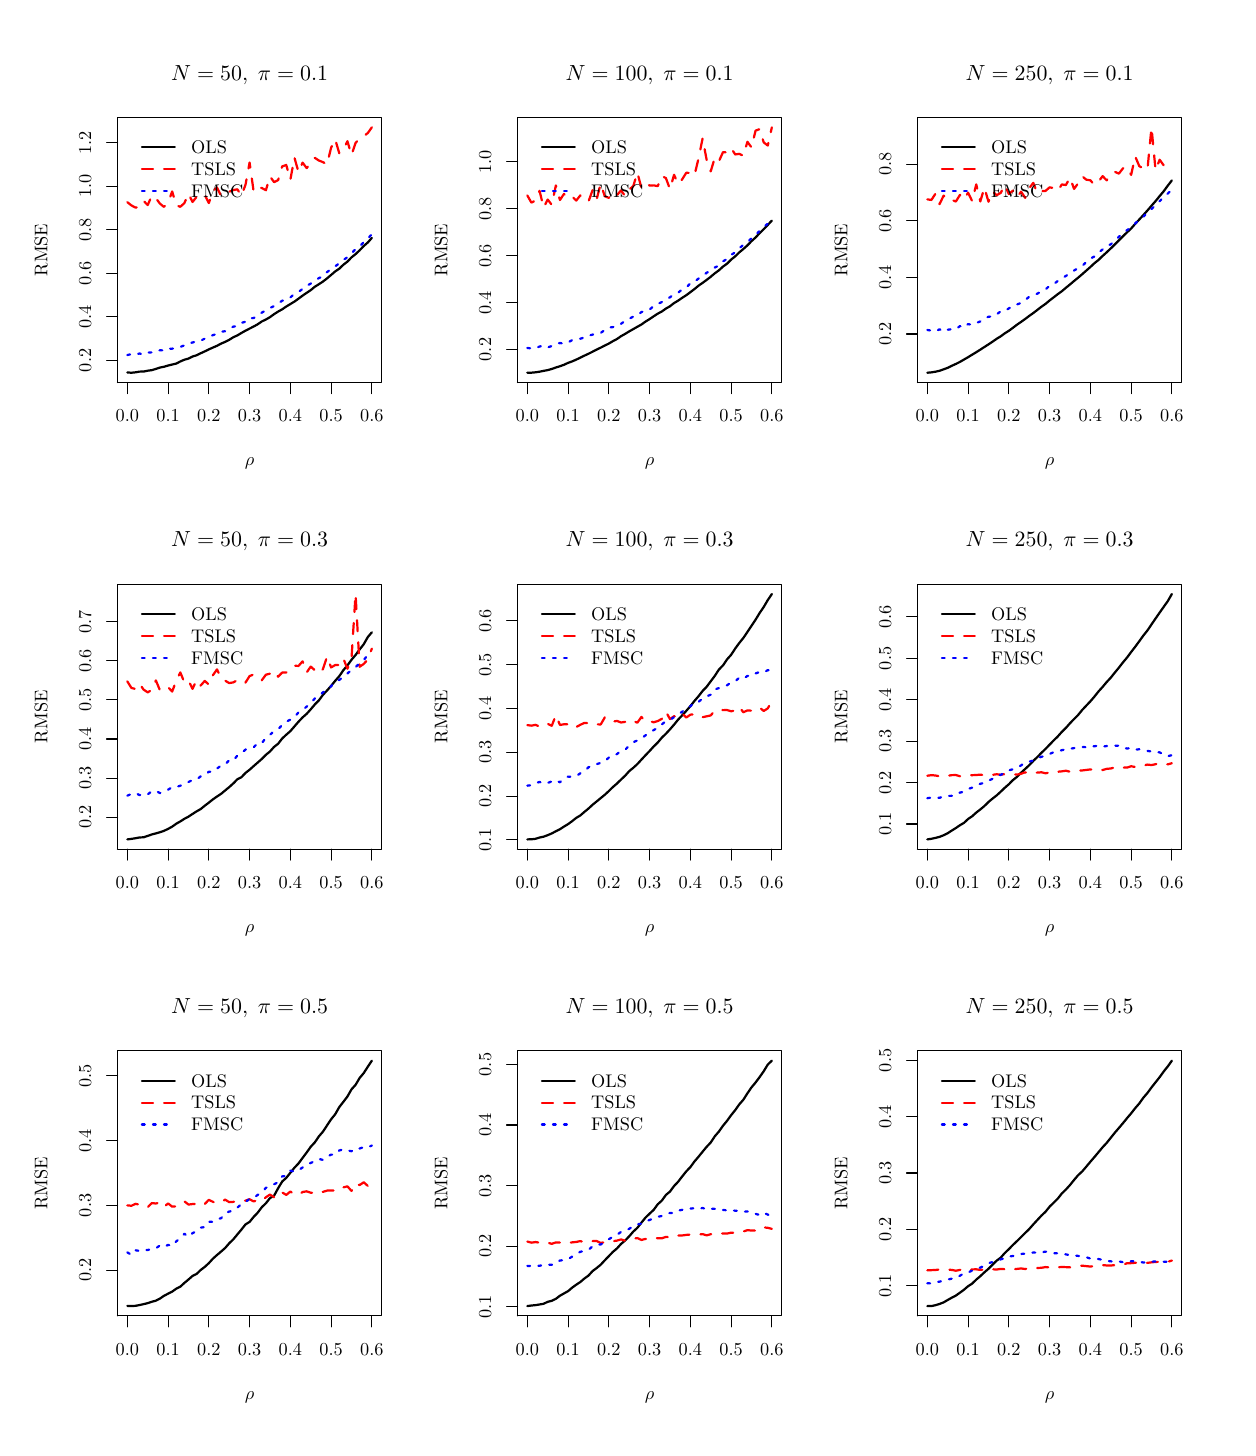
\begin{tikzpicture}[x=1pt,y=1pt]
\definecolor[named]{fillColor}{rgb}{1.00,1.00,1.00}
\path[use as bounding box,fill=fillColor,fill opacity=0.00] (0,0) rectangle (433.62,505.89);
\begin{scope}
\path[clip] ( 32.47,377.65) rectangle (127.91,473.42);
\definecolor[named]{drawColor}{rgb}{0.00,0.00,0.00}

\path[draw=drawColor,line width= 0.8pt,line join=round,line cap=round] ( 36.01,381.30) --
	( 37.48,381.20) --
	( 38.95,381.34) --
	( 40.42,381.60) --
	( 41.90,381.62) --
	( 43.37,381.93) --
	( 44.84,382.13) --
	( 46.32,382.57) --
	( 47.79,383.07) --
	( 49.26,383.36) --
	( 50.73,383.80) --
	( 52.21,384.16) --
	( 53.68,384.50) --
	( 55.15,385.27) --
	( 56.63,385.90) --
	( 58.10,386.31) --
	( 59.57,387.06) --
	( 61.04,387.50) --
	( 62.52,388.24) --
	( 63.99,388.91) --
	( 65.46,389.63) --
	( 66.93,390.29) --
	( 68.41,390.93) --
	( 69.88,391.72) --
	( 71.35,392.34) --
	( 72.83,393.09) --
	( 74.30,394.02) --
	( 75.77,394.69) --
	( 77.24,395.57) --
	( 78.72,396.40) --
	( 80.19,397.15) --
	( 81.66,397.90) --
	( 83.14,398.72) --
	( 84.61,399.73) --
	( 86.08,400.44) --
	( 87.55,401.28) --
	( 89.03,402.36) --
	( 90.50,403.30) --
	( 91.97,404.12) --
	( 93.44,405.11) --
	( 94.92,406.02) --
	( 96.39,406.90) --
	( 97.86,407.96) --
	( 99.34,409.06) --
	(100.81,410.07) --
	(102.28,411.05) --
	(103.75,412.26) --
	(105.23,413.18) --
	(106.70,414.15) --
	(108.17,415.29) --
	(109.65,416.54) --
	(111.12,417.80) --
	(112.59,418.79) --
	(114.06,420.21) --
	(115.54,421.34) --
	(117.01,422.88) --
	(118.48,424.06) --
	(119.95,425.43) --
	(121.43,426.99) --
	(122.90,428.26) --
	(124.37,429.94);
\end{scope}
\begin{scope}
\path[clip] (  0.00,  0.00) rectangle (433.62,505.89);
\definecolor[named]{drawColor}{rgb}{0.00,0.00,0.00}

\path[draw=drawColor,line width= 0.4pt,line join=round,line cap=round] ( 36.01,377.65) -- (124.37,377.65);

\path[draw=drawColor,line width= 0.4pt,line join=round,line cap=round] ( 36.01,377.65) -- ( 36.01,373.69);

\path[draw=drawColor,line width= 0.4pt,line join=round,line cap=round] ( 50.73,377.65) -- ( 50.73,373.69);

\path[draw=drawColor,line width= 0.4pt,line join=round,line cap=round] ( 65.46,377.65) -- ( 65.46,373.69);

\path[draw=drawColor,line width= 0.4pt,line join=round,line cap=round] ( 80.19,377.65) -- ( 80.19,373.69);

\path[draw=drawColor,line width= 0.4pt,line join=round,line cap=round] ( 94.92,377.65) -- ( 94.92,373.69);

\path[draw=drawColor,line width= 0.4pt,line join=round,line cap=round] (109.65,377.65) -- (109.65,373.69);

\path[draw=drawColor,line width= 0.4pt,line join=round,line cap=round] (124.37,377.65) -- (124.37,373.69);

\node[text=drawColor,anchor=base,inner sep=0pt, outer sep=0pt, scale=  0.66] at ( 36.01,363.40) {0.0};

\node[text=drawColor,anchor=base,inner sep=0pt, outer sep=0pt, scale=  0.66] at ( 50.73,363.40) {0.1};

\node[text=drawColor,anchor=base,inner sep=0pt, outer sep=0pt, scale=  0.66] at ( 65.46,363.40) {0.2};

\node[text=drawColor,anchor=base,inner sep=0pt, outer sep=0pt, scale=  0.66] at ( 80.19,363.40) {0.3};

\node[text=drawColor,anchor=base,inner sep=0pt, outer sep=0pt, scale=  0.66] at ( 94.92,363.40) {0.4};

\node[text=drawColor,anchor=base,inner sep=0pt, outer sep=0pt, scale=  0.66] at (109.65,363.40) {0.5};

\node[text=drawColor,anchor=base,inner sep=0pt, outer sep=0pt, scale=  0.66] at (124.37,363.40) {0.6};

\path[draw=drawColor,line width= 0.4pt,line join=round,line cap=round] ( 32.47,385.64) -- ( 32.47,464.32);

\path[draw=drawColor,line width= 0.4pt,line join=round,line cap=round] ( 32.47,385.64) -- ( 28.51,385.64);

\path[draw=drawColor,line width= 0.4pt,line join=round,line cap=round] ( 32.47,401.37) -- ( 28.51,401.37);

\path[draw=drawColor,line width= 0.4pt,line join=round,line cap=round] ( 32.47,417.11) -- ( 28.51,417.11);

\path[draw=drawColor,line width= 0.4pt,line join=round,line cap=round] ( 32.47,432.85) -- ( 28.51,432.85);

\path[draw=drawColor,line width= 0.4pt,line join=round,line cap=round] ( 32.47,448.58) -- ( 28.51,448.58);

\path[draw=drawColor,line width= 0.4pt,line join=round,line cap=round] ( 32.47,464.32) -- ( 28.51,464.32);

\node[text=drawColor,rotate= 90.00,anchor=base,inner sep=0pt, outer sep=0pt, scale=  0.66] at ( 22.97,385.64) {0.2};

\node[text=drawColor,rotate= 90.00,anchor=base,inner sep=0pt, outer sep=0pt, scale=  0.66] at ( 22.97,401.37) {0.4};

\node[text=drawColor,rotate= 90.00,anchor=base,inner sep=0pt, outer sep=0pt, scale=  0.66] at ( 22.97,417.11) {0.6};

\node[text=drawColor,rotate= 90.00,anchor=base,inner sep=0pt, outer sep=0pt, scale=  0.66] at ( 22.97,432.85) {0.8};

\node[text=drawColor,rotate= 90.00,anchor=base,inner sep=0pt, outer sep=0pt, scale=  0.66] at ( 22.97,448.58) {1.0};

\node[text=drawColor,rotate= 90.00,anchor=base,inner sep=0pt, outer sep=0pt, scale=  0.66] at ( 22.97,464.32) {1.2};

\path[draw=drawColor,line width= 0.4pt,line join=round,line cap=round] ( 32.47,377.65) --
	(127.91,377.65) --
	(127.91,473.42) --
	( 32.47,473.42) --
	( 32.47,377.65);
\end{scope}
\begin{scope}
\path[clip] (  0.00,337.26) rectangle (144.54,505.89);
\definecolor[named]{drawColor}{rgb}{0.00,0.00,0.00}

\node[text=drawColor,anchor=base,inner sep=0pt, outer sep=0pt, scale=  0.79] at ( 80.19,486.92) {\bfseries $N=50, \;\pi=0.1$};

\node[text=drawColor,anchor=base,inner sep=0pt, outer sep=0pt, scale=  0.66] at ( 80.19,347.56) {$\rho$};

\node[text=drawColor,rotate= 90.00,anchor=base,inner sep=0pt, outer sep=0pt, scale=  0.66] at (  7.13,425.53) {RMSE};
\end{scope}
\begin{scope}
\path[clip] ( 32.47,377.65) rectangle (127.91,473.42);
\definecolor[named]{drawColor}{rgb}{1.00,0.00,0.00}

\path[draw=drawColor,line width= 0.8pt,dash pattern=on 4pt off 4pt ,line join=round,line cap=round] ( 36.01,442.82) --
	( 37.48,441.66) --
	( 38.95,440.86) --
	( 40.42,441.14) --
	( 41.90,443.29) --
	( 43.37,441.77) --
	( 44.84,445.14) --
	( 46.32,444.29) --
	( 47.79,442.31) --
	( 49.26,441.12) --
	( 50.73,442.62) --
	( 52.21,446.71) --
	( 53.68,441.70) --
	( 55.15,441.16) --
	( 56.63,442.50) --
	( 58.10,445.92) --
	( 59.57,442.91) --
	( 61.04,444.73) --
	( 62.52,444.50) --
	( 63.99,445.47) --
	( 65.46,442.51) --
	( 66.93,446.89) --
	( 68.41,448.11) --
	( 69.88,445.18) --
	( 71.35,446.35) --
	( 72.83,446.61) --
	( 74.30,447.20) --
	( 75.77,447.48) --
	( 77.24,445.14) --
	( 78.72,449.16) --
	( 80.19,457.16) --
	( 81.66,446.64) --
	( 83.14,447.98) --
	( 84.61,447.95) --
	( 86.08,447.14) --
	( 87.55,452.15) --
	( 89.03,450.08) --
	( 90.50,450.78) --
	( 91.97,455.76) --
	( 93.44,456.27) --
	( 94.92,450.94) --
	( 96.39,458.93) --
	( 97.86,453.71) --
	( 99.34,457.12) --
	(100.81,455.15) --
	(102.28,456.78) --
	(103.75,458.84) --
	(105.23,457.88) --
	(106.70,457.30) --
	(108.17,456.45) --
	(109.65,462.55) --
	(111.12,465.54) --
	(112.59,460.53) --
	(114.06,461.70) --
	(115.54,464.87) --
	(117.01,459.83) --
	(118.48,464.22) --
	(119.95,465.97) --
	(121.43,466.66) --
	(122.90,467.80) --
	(124.37,469.87);
\definecolor[named]{drawColor}{rgb}{0.00,0.00,1.00}

\path[draw=drawColor,line width= 0.8pt,dash pattern=on 1pt off 3pt ,line join=round,line cap=round] ( 36.01,387.59) --
	( 37.48,387.92) --
	( 38.95,387.80) --
	( 40.42,388.14) --
	( 41.90,387.76) --
	( 43.37,388.44) --
	( 44.84,388.57) --
	( 46.32,388.87) --
	( 47.79,389.30) --
	( 49.26,389.26) --
	( 50.73,389.91) --
	( 52.21,389.89) --
	( 53.68,390.14) --
	( 55.15,390.51) --
	( 56.63,391.10) --
	( 58.10,391.74) --
	( 59.57,392.12) --
	( 61.04,392.59) --
	( 62.52,392.80) --
	( 63.99,393.52) --
	( 65.46,394.08) --
	( 66.93,394.78) --
	( 68.41,395.26) --
	( 69.88,395.98) --
	( 71.35,396.21) --
	( 72.83,396.99) --
	( 74.30,397.85) --
	( 75.77,398.11) --
	( 77.24,399.22) --
	( 78.72,399.62) --
	( 80.19,400.88) --
	( 81.66,400.95) --
	( 83.14,401.93) --
	( 84.61,402.92) --
	( 86.08,403.75) --
	( 87.55,404.60) --
	( 89.03,405.27) --
	( 90.50,406.24) --
	( 91.97,407.22) --
	( 93.44,407.69) --
	( 94.92,408.42) --
	( 96.39,409.67) --
	( 97.86,410.35) --
	( 99.34,411.51) --
	(100.81,412.62) --
	(102.28,413.40) --
	(103.75,414.43) --
	(105.23,415.40) --
	(106.70,416.02) --
	(108.17,417.54) --
	(109.65,418.68) --
	(111.12,419.66) --
	(112.59,420.70) --
	(114.06,421.95) --
	(115.54,422.93) --
	(117.01,424.37) --
	(118.48,425.81) --
	(119.95,426.78) --
	(121.43,428.42) --
	(122.90,429.72) --
	(124.37,431.28);
\definecolor[named]{drawColor}{rgb}{0.00,0.00,0.00}

\path[draw=drawColor,line width= 0.8pt,line join=round,line cap=round] ( 41.28,462.63) -- ( 53.16,462.63);
\definecolor[named]{drawColor}{rgb}{1.00,0.00,0.00}

\path[draw=drawColor,line width= 0.8pt,dash pattern=on 4pt off 4pt ,line join=round,line cap=round] ( 41.28,454.71) -- ( 53.16,454.71);
\definecolor[named]{drawColor}{rgb}{0.00,0.00,1.00}

\path[draw=drawColor,line width= 0.8pt,dash pattern=on 1pt off 3pt ,line join=round,line cap=round] ( 41.28,446.79) -- ( 53.16,446.79);
\definecolor[named]{drawColor}{rgb}{0.00,0.00,0.00}

\node[text=drawColor,anchor=base west,inner sep=0pt, outer sep=0pt, scale=  0.66] at ( 59.10,460.35) {OLS};

\node[text=drawColor,anchor=base west,inner sep=0pt, outer sep=0pt, scale=  0.66] at ( 59.10,452.43) {TSLS};

\node[text=drawColor,anchor=base west,inner sep=0pt, outer sep=0pt, scale=  0.66] at ( 59.10,444.51) {FMSC};
\end{scope}
\begin{scope}
\path[clip] ( 32.47,209.02) rectangle (127.91,304.79);
\definecolor[named]{drawColor}{rgb}{0.00,0.00,0.00}

\path[draw=drawColor,line width= 0.8pt,line join=round,line cap=round] ( 36.01,212.57) --
	( 37.48,212.76) --
	( 38.95,212.99) --
	( 40.42,213.27) --
	( 41.90,213.33) --
	( 43.37,213.83) --
	( 44.84,214.35) --
	( 46.32,214.74) --
	( 47.79,215.16) --
	( 49.26,215.66) --
	( 50.73,216.37) --
	( 52.21,217.17) --
	( 53.68,218.23) --
	( 55.15,219.06) --
	( 56.63,220.01) --
	( 58.10,220.78) --
	( 59.57,221.76) --
	( 61.04,222.70) --
	( 62.52,223.53) --
	( 63.99,224.75) --
	( 65.46,225.85) --
	( 66.93,227.03) --
	( 68.41,228.07) --
	( 69.88,229.03) --
	( 71.35,230.25) --
	( 72.83,231.47) --
	( 74.30,232.80) --
	( 75.77,234.29) --
	( 77.24,235.04) --
	( 78.72,236.60) --
	( 80.19,237.74) --
	( 81.66,239.06) --
	( 83.14,240.35) --
	( 84.61,241.64) --
	( 86.08,243.13) --
	( 87.55,244.33) --
	( 89.03,245.99) --
	( 90.50,247.13) --
	( 91.97,249.03) --
	( 93.44,250.40) --
	( 94.92,251.69) --
	( 96.39,253.39) --
	( 97.86,255.09) --
	( 99.34,256.65) --
	(100.81,257.94) --
	(102.28,259.57) --
	(103.75,261.31) --
	(105.23,262.81) --
	(106.70,264.81) --
	(108.17,266.37) --
	(109.65,268.05) --
	(111.12,269.87) --
	(112.59,271.54) --
	(114.06,273.70) --
	(115.54,275.43) --
	(117.01,277.47) --
	(118.48,279.20) --
	(119.95,281.22) --
	(121.43,283.09) --
	(122.90,285.68) --
	(124.37,287.40);
\end{scope}
\begin{scope}
\path[clip] (  0.00,  0.00) rectangle (433.62,505.89);
\definecolor[named]{drawColor}{rgb}{0.00,0.00,0.00}

\path[draw=drawColor,line width= 0.4pt,line join=round,line cap=round] ( 36.01,209.02) -- (124.37,209.02);

\path[draw=drawColor,line width= 0.4pt,line join=round,line cap=round] ( 36.01,209.02) -- ( 36.01,205.06);

\path[draw=drawColor,line width= 0.4pt,line join=round,line cap=round] ( 50.73,209.02) -- ( 50.73,205.06);

\path[draw=drawColor,line width= 0.4pt,line join=round,line cap=round] ( 65.46,209.02) -- ( 65.46,205.06);

\path[draw=drawColor,line width= 0.4pt,line join=round,line cap=round] ( 80.19,209.02) -- ( 80.19,205.06);

\path[draw=drawColor,line width= 0.4pt,line join=round,line cap=round] ( 94.92,209.02) -- ( 94.92,205.06);

\path[draw=drawColor,line width= 0.4pt,line join=round,line cap=round] (109.65,209.02) -- (109.65,205.06);

\path[draw=drawColor,line width= 0.4pt,line join=round,line cap=round] (124.37,209.02) -- (124.37,205.06);

\node[text=drawColor,anchor=base,inner sep=0pt, outer sep=0pt, scale=  0.66] at ( 36.01,194.77) {0.0};

\node[text=drawColor,anchor=base,inner sep=0pt, outer sep=0pt, scale=  0.66] at ( 50.73,194.77) {0.1};

\node[text=drawColor,anchor=base,inner sep=0pt, outer sep=0pt, scale=  0.66] at ( 65.46,194.77) {0.2};

\node[text=drawColor,anchor=base,inner sep=0pt, outer sep=0pt, scale=  0.66] at ( 80.19,194.77) {0.3};

\node[text=drawColor,anchor=base,inner sep=0pt, outer sep=0pt, scale=  0.66] at ( 94.92,194.77) {0.4};

\node[text=drawColor,anchor=base,inner sep=0pt, outer sep=0pt, scale=  0.66] at (109.65,194.77) {0.5};

\node[text=drawColor,anchor=base,inner sep=0pt, outer sep=0pt, scale=  0.66] at (124.37,194.77) {0.6};

\path[draw=drawColor,line width= 0.4pt,line join=round,line cap=round] ( 32.47,220.61) -- ( 32.47,291.20);

\path[draw=drawColor,line width= 0.4pt,line join=round,line cap=round] ( 32.47,220.61) -- ( 28.51,220.61);

\path[draw=drawColor,line width= 0.4pt,line join=round,line cap=round] ( 32.47,234.73) -- ( 28.51,234.73);

\path[draw=drawColor,line width= 0.4pt,line join=round,line cap=round] ( 32.47,248.85) -- ( 28.51,248.85);

\path[draw=drawColor,line width= 0.4pt,line join=round,line cap=round] ( 32.47,262.97) -- ( 28.51,262.97);

\path[draw=drawColor,line width= 0.4pt,line join=round,line cap=round] ( 32.47,277.08) -- ( 28.51,277.08);

\path[draw=drawColor,line width= 0.4pt,line join=round,line cap=round] ( 32.47,291.20) -- ( 28.51,291.20);

\node[text=drawColor,rotate= 90.00,anchor=base,inner sep=0pt, outer sep=0pt, scale=  0.66] at ( 22.97,220.61) {0.2};

\node[text=drawColor,rotate= 90.00,anchor=base,inner sep=0pt, outer sep=0pt, scale=  0.66] at ( 22.97,234.73) {0.3};

\node[text=drawColor,rotate= 90.00,anchor=base,inner sep=0pt, outer sep=0pt, scale=  0.66] at ( 22.97,248.85) {0.4};

\node[text=drawColor,rotate= 90.00,anchor=base,inner sep=0pt, outer sep=0pt, scale=  0.66] at ( 22.97,262.97) {0.5};

\node[text=drawColor,rotate= 90.00,anchor=base,inner sep=0pt, outer sep=0pt, scale=  0.66] at ( 22.97,277.08) {0.6};

\node[text=drawColor,rotate= 90.00,anchor=base,inner sep=0pt, outer sep=0pt, scale=  0.66] at ( 22.97,291.20) {0.7};

\path[draw=drawColor,line width= 0.4pt,line join=round,line cap=round] ( 32.47,209.02) --
	(127.91,209.02) --
	(127.91,304.79) --
	( 32.47,304.79) --
	( 32.47,209.02);
\end{scope}
\begin{scope}
\path[clip] (  0.00,168.63) rectangle (144.54,337.26);
\definecolor[named]{drawColor}{rgb}{0.00,0.00,0.00}

\node[text=drawColor,anchor=base,inner sep=0pt, outer sep=0pt, scale=  0.79] at ( 80.19,318.29) {\bfseries $N=50, \;\pi=0.3$};

\node[text=drawColor,anchor=base,inner sep=0pt, outer sep=0pt, scale=  0.66] at ( 80.19,178.93) {$\rho$};

\node[text=drawColor,rotate= 90.00,anchor=base,inner sep=0pt, outer sep=0pt, scale=  0.66] at (  7.13,256.90) {RMSE};
\end{scope}
\begin{scope}
\path[clip] ( 32.47,209.02) rectangle (127.91,304.79);
\definecolor[named]{drawColor}{rgb}{1.00,0.00,0.00}

\path[draw=drawColor,line width= 0.8pt,dash pattern=on 4pt off 4pt ,line join=round,line cap=round] ( 36.01,269.67) --
	( 37.48,267.31) --
	( 38.95,266.92) --
	( 40.42,268.79) --
	( 41.90,266.68) --
	( 43.37,265.70) --
	( 44.84,266.58) --
	( 46.32,270.03) --
	( 47.79,266.46) --
	( 49.26,266.84) --
	( 50.73,267.60) --
	( 52.21,265.99) --
	( 53.68,269.87) --
	( 55.15,272.92) --
	( 56.63,269.29) --
	( 58.10,269.97) --
	( 59.57,266.96) --
	( 61.04,270.17) --
	( 62.52,268.18) --
	( 63.99,269.84) --
	( 65.46,268.51) --
	( 66.93,271.89) --
	( 68.41,274.01) --
	( 69.88,270.79) --
	( 71.35,269.93) --
	( 72.83,269.05) --
	( 74.30,269.31) --
	( 75.77,270.09) --
	( 77.24,270.39) --
	( 78.72,269.26) --
	( 80.19,271.59) --
	( 81.66,272.17) --
	( 83.14,271.25) --
	( 84.61,270.10) --
	( 86.08,272.08) --
	( 87.55,272.46) --
	( 89.03,273.42) --
	( 90.50,271.36) --
	( 91.97,272.85) --
	( 93.44,272.90) --
	( 94.92,273.82) --
	( 96.39,275.32) --
	( 97.86,275.25) --
	( 99.34,276.91) --
	(100.81,272.89) --
	(102.28,275.01) --
	(103.75,273.71) --
	(105.23,272.57) --
	(106.70,274.10) --
	(108.17,278.61) --
	(109.65,274.70) --
	(111.12,275.57) --
	(112.59,275.56) --
	(114.06,277.96) --
	(115.54,274.23) --
	(117.01,277.89) --
	(118.48,301.24) --
	(119.95,274.94) --
	(121.43,275.97) --
	(122.90,277.58) --
	(124.37,281.51);
\definecolor[named]{drawColor}{rgb}{0.00,0.00,1.00}

\path[draw=drawColor,line width= 0.8pt,dash pattern=on 1pt off 3pt ,line join=round,line cap=round] ( 36.01,228.37) --
	( 37.48,228.99) --
	( 38.95,229.32) --
	( 40.42,228.57) --
	( 41.90,229.06) --
	( 43.37,228.83) --
	( 44.84,229.98) --
	( 46.32,230.10) --
	( 47.79,229.31) --
	( 49.26,229.90) --
	( 50.73,230.53) --
	( 52.21,231.46) --
	( 53.68,231.50) --
	( 55.15,231.96) --
	( 56.63,232.58) --
	( 58.10,233.31) --
	( 59.57,234.02) --
	( 61.04,234.23) --
	( 62.52,235.35) --
	( 63.99,235.67) --
	( 65.46,237.02) --
	( 66.93,237.04) --
	( 68.41,238.16) --
	( 69.88,239.26) --
	( 71.35,239.61) --
	( 72.83,241.21) --
	( 74.30,241.03) --
	( 75.77,242.87) --
	( 77.24,243.68) --
	( 78.72,245.03) --
	( 80.19,245.42) --
	( 81.66,245.84) --
	( 83.14,247.43) --
	( 84.61,247.36) --
	( 86.08,249.27) --
	( 87.55,250.34) --
	( 89.03,251.72) --
	( 90.50,252.32) --
	( 91.97,253.96) --
	( 93.44,255.07) --
	( 94.92,255.86) --
	( 96.39,256.72) --
	( 97.86,258.47) --
	( 99.34,259.26) --
	(100.81,260.57) --
	(102.28,261.81) --
	(103.75,263.48) --
	(105.23,264.30) --
	(106.70,265.74) --
	(108.17,266.24) --
	(109.65,267.93) --
	(111.12,269.49) --
	(112.59,270.17) --
	(114.06,271.39) --
	(115.54,272.50) --
	(117.01,273.87) --
	(118.48,274.78) --
	(119.95,276.29) --
	(121.43,277.32) --
	(122.90,279.28) --
	(124.37,280.00);
\definecolor[named]{drawColor}{rgb}{0.00,0.00,0.00}

\path[draw=drawColor,line width= 0.8pt,line join=round,line cap=round] ( 41.28,294.00) -- ( 53.16,294.00);
\definecolor[named]{drawColor}{rgb}{1.00,0.00,0.00}

\path[draw=drawColor,line width= 0.8pt,dash pattern=on 4pt off 4pt ,line join=round,line cap=round] ( 41.28,286.08) -- ( 53.16,286.08);
\definecolor[named]{drawColor}{rgb}{0.00,0.00,1.00}

\path[draw=drawColor,line width= 0.8pt,dash pattern=on 1pt off 3pt ,line join=round,line cap=round] ( 41.28,278.16) -- ( 53.16,278.16);
\definecolor[named]{drawColor}{rgb}{0.00,0.00,0.00}

\node[text=drawColor,anchor=base west,inner sep=0pt, outer sep=0pt, scale=  0.66] at ( 59.10,291.72) {OLS};

\node[text=drawColor,anchor=base west,inner sep=0pt, outer sep=0pt, scale=  0.66] at ( 59.10,283.80) {TSLS};

\node[text=drawColor,anchor=base west,inner sep=0pt, outer sep=0pt, scale=  0.66] at ( 59.10,275.88) {FMSC};
\end{scope}
\begin{scope}
\path[clip] ( 32.47, 40.39) rectangle (127.91,136.16);
\definecolor[named]{drawColor}{rgb}{0.00,0.00,0.00}

\path[draw=drawColor,line width= 0.8pt,line join=round,line cap=round] ( 36.01, 43.99) --
	( 37.48, 43.94) --
	( 38.95, 44.03) --
	( 40.42, 44.31) --
	( 41.90, 44.64) --
	( 43.37, 45.00) --
	( 44.84, 45.50) --
	( 46.32, 45.88) --
	( 47.79, 46.65) --
	( 49.26, 47.65) --
	( 50.73, 48.41) --
	( 52.21, 49.17) --
	( 53.68, 50.21) --
	( 55.15, 50.95) --
	( 56.63, 52.31) --
	( 58.10, 53.53) --
	( 59.57, 54.82) --
	( 61.04, 55.55) --
	( 62.52, 56.98) --
	( 63.99, 58.09) --
	( 65.46, 59.45) --
	( 66.93, 61.06) --
	( 68.41, 62.39) --
	( 69.88, 63.63) --
	( 71.35, 64.92) --
	( 72.83, 66.63) --
	( 74.30, 68.04) --
	( 75.77, 69.83) --
	( 77.24, 71.58) --
	( 78.72, 73.45) --
	( 80.19, 74.36) --
	( 81.66, 76.16) --
	( 83.14, 77.70) --
	( 84.61, 79.68) --
	( 86.08, 81.08) --
	( 87.55, 82.96) --
	( 89.03, 83.83) --
	( 90.50, 86.52) --
	( 91.97, 88.94) --
	( 93.44, 90.28) --
	( 94.92, 92.11) --
	( 96.39, 93.92) --
	( 97.86, 95.48) --
	( 99.34, 97.47) --
	(100.81, 99.43) --
	(102.28,101.50) --
	(103.75,103.08) --
	(105.23,105.26) --
	(106.70,106.97) --
	(108.17,109.21) --
	(109.65,111.44) --
	(111.12,113.25) --
	(112.59,115.83) --
	(114.06,117.71) --
	(115.54,119.66) --
	(117.01,122.24) --
	(118.48,123.88) --
	(119.95,126.35) --
	(121.43,128.13) --
	(122.90,130.41) --
	(124.37,132.61);
\end{scope}
\begin{scope}
\path[clip] (  0.00,  0.00) rectangle (433.62,505.89);
\definecolor[named]{drawColor}{rgb}{0.00,0.00,0.00}

\path[draw=drawColor,line width= 0.4pt,line join=round,line cap=round] ( 36.01, 40.39) -- (124.37, 40.39);

\path[draw=drawColor,line width= 0.4pt,line join=round,line cap=round] ( 36.01, 40.39) -- ( 36.01, 36.43);

\path[draw=drawColor,line width= 0.4pt,line join=round,line cap=round] ( 50.73, 40.39) -- ( 50.73, 36.43);

\path[draw=drawColor,line width= 0.4pt,line join=round,line cap=round] ( 65.46, 40.39) -- ( 65.46, 36.43);

\path[draw=drawColor,line width= 0.4pt,line join=round,line cap=round] ( 80.19, 40.39) -- ( 80.19, 36.43);

\path[draw=drawColor,line width= 0.4pt,line join=round,line cap=round] ( 94.92, 40.39) -- ( 94.92, 36.43);

\path[draw=drawColor,line width= 0.4pt,line join=round,line cap=round] (109.65, 40.39) -- (109.65, 36.43);

\path[draw=drawColor,line width= 0.4pt,line join=round,line cap=round] (124.37, 40.39) -- (124.37, 36.43);

\node[text=drawColor,anchor=base,inner sep=0pt, outer sep=0pt, scale=  0.66] at ( 36.01, 26.14) {0.0};

\node[text=drawColor,anchor=base,inner sep=0pt, outer sep=0pt, scale=  0.66] at ( 50.73, 26.14) {0.1};

\node[text=drawColor,anchor=base,inner sep=0pt, outer sep=0pt, scale=  0.66] at ( 65.46, 26.14) {0.2};

\node[text=drawColor,anchor=base,inner sep=0pt, outer sep=0pt, scale=  0.66] at ( 80.19, 26.14) {0.3};

\node[text=drawColor,anchor=base,inner sep=0pt, outer sep=0pt, scale=  0.66] at ( 94.92, 26.14) {0.4};

\node[text=drawColor,anchor=base,inner sep=0pt, outer sep=0pt, scale=  0.66] at (109.65, 26.14) {0.5};

\node[text=drawColor,anchor=base,inner sep=0pt, outer sep=0pt, scale=  0.66] at (124.37, 26.14) {0.6};

\path[draw=drawColor,line width= 0.4pt,line join=round,line cap=round] ( 32.47, 56.92) -- ( 32.47,127.15);

\path[draw=drawColor,line width= 0.4pt,line join=round,line cap=round] ( 32.47, 56.92) -- ( 28.51, 56.92);

\path[draw=drawColor,line width= 0.4pt,line join=round,line cap=round] ( 32.47, 80.33) -- ( 28.51, 80.33);

\path[draw=drawColor,line width= 0.4pt,line join=round,line cap=round] ( 32.47,103.74) -- ( 28.51,103.74);

\path[draw=drawColor,line width= 0.4pt,line join=round,line cap=round] ( 32.47,127.15) -- ( 28.51,127.15);

\node[text=drawColor,rotate= 90.00,anchor=base,inner sep=0pt, outer sep=0pt, scale=  0.66] at ( 22.97, 56.92) {0.2};

\node[text=drawColor,rotate= 90.00,anchor=base,inner sep=0pt, outer sep=0pt, scale=  0.66] at ( 22.97, 80.33) {0.3};

\node[text=drawColor,rotate= 90.00,anchor=base,inner sep=0pt, outer sep=0pt, scale=  0.66] at ( 22.97,103.74) {0.4};

\node[text=drawColor,rotate= 90.00,anchor=base,inner sep=0pt, outer sep=0pt, scale=  0.66] at ( 22.97,127.15) {0.5};

\path[draw=drawColor,line width= 0.4pt,line join=round,line cap=round] ( 32.47, 40.39) --
	(127.91, 40.39) --
	(127.91,136.16) --
	( 32.47,136.16) --
	( 32.47, 40.39);
\end{scope}
\begin{scope}
\path[clip] (  0.00,  0.00) rectangle (144.54,168.63);
\definecolor[named]{drawColor}{rgb}{0.00,0.00,0.00}

\node[text=drawColor,anchor=base,inner sep=0pt, outer sep=0pt, scale=  0.79] at ( 80.19,149.66) {\bfseries $N=50, \;\pi=0.5$};

\node[text=drawColor,anchor=base,inner sep=0pt, outer sep=0pt, scale=  0.66] at ( 80.19, 10.30) {$\rho$};

\node[text=drawColor,rotate= 90.00,anchor=base,inner sep=0pt, outer sep=0pt, scale=  0.66] at (  7.13, 88.27) {RMSE};
\end{scope}
\begin{scope}
\path[clip] ( 32.47, 40.39) rectangle (127.91,136.16);
\definecolor[named]{drawColor}{rgb}{1.00,0.00,0.00}

\path[draw=drawColor,line width= 0.8pt,dash pattern=on 4pt off 4pt ,line join=round,line cap=round] ( 36.01, 80.33) --
	( 37.48, 80.18) --
	( 38.95, 80.89) --
	( 40.42, 80.57) --
	( 41.90, 80.58) --
	( 43.37, 79.67) --
	( 44.84, 81.16) --
	( 46.32, 81.00) --
	( 47.79, 81.38) --
	( 49.26, 79.77) --
	( 50.73, 81.04) --
	( 52.21, 79.87) --
	( 53.68, 79.98) --
	( 55.15, 80.84) --
	( 56.63, 81.78) --
	( 58.10, 80.62) --
	( 59.57, 80.80) --
	( 61.04, 80.86) --
	( 62.52, 81.58) --
	( 63.99, 80.84) --
	( 65.46, 82.33) --
	( 66.93, 81.61) --
	( 68.41, 81.12) --
	( 69.88, 81.46) --
	( 71.35, 82.40) --
	( 72.83, 81.49) --
	( 74.30, 81.60) --
	( 75.77, 81.76) --
	( 77.24, 81.86) --
	( 78.72, 82.05) --
	( 80.19, 82.54) --
	( 81.66, 81.76) --
	( 83.14, 82.21) --
	( 84.61, 81.85) --
	( 86.08, 83.26) --
	( 87.55, 84.22) --
	( 89.03, 83.30) --
	( 90.50, 83.18) --
	( 91.97, 85.00) --
	( 93.44, 84.11) --
	( 94.92, 85.32) --
	( 96.39, 84.30) --
	( 97.86, 84.12) --
	( 99.34, 85.15) --
	(100.81, 85.41) --
	(102.28, 84.90) --
	(103.75, 84.92) --
	(105.23, 85.47) --
	(106.70, 85.20) --
	(108.17, 85.66) --
	(109.65, 85.73) --
	(111.12, 85.66) --
	(112.59, 86.79) --
	(114.06, 86.82) --
	(115.54, 87.21) --
	(117.01, 85.55) --
	(118.48, 88.24) --
	(119.95, 87.68) --
	(121.43, 88.67) --
	(122.90, 87.37) --
	(124.37, 88.45);
\definecolor[named]{drawColor}{rgb}{0.00,0.00,1.00}

\path[draw=drawColor,line width= 0.8pt,dash pattern=on 1pt off 3pt ,line join=round,line cap=round] ( 36.01, 63.34) --
	( 37.48, 62.44) --
	( 38.95, 64.10) --
	( 40.42, 63.88) --
	( 41.90, 64.31) --
	( 43.37, 64.16) --
	( 44.84, 64.74) --
	( 46.32, 64.80) --
	( 47.79, 65.86) --
	( 49.26, 65.27) --
	( 50.73, 66.05) --
	( 52.21, 65.63) --
	( 53.68, 67.33) --
	( 55.15, 68.39) --
	( 56.63, 70.09) --
	( 58.10, 68.92) --
	( 59.57, 70.30) --
	( 61.04, 70.97) --
	( 62.52, 72.29) --
	( 63.99, 72.49) --
	( 65.46, 74.40) --
	( 66.93, 74.38) --
	( 68.41, 75.32) --
	( 69.88, 75.66) --
	( 71.35, 77.48) --
	( 72.83, 78.10) --
	( 74.30, 78.39) --
	( 75.77, 79.51) --
	( 77.24, 80.81) --
	( 78.72, 81.45) --
	( 80.19, 82.78) --
	( 81.66, 82.93) --
	( 83.14, 84.16) --
	( 84.61, 84.90) --
	( 86.08, 86.68) --
	( 87.55, 87.23) --
	( 89.03, 87.95) --
	( 90.50, 88.69) --
	( 91.97, 90.80) --
	( 93.44, 90.99) --
	( 94.92, 92.87) --
	( 96.39, 92.52) --
	( 97.86, 93.00) --
	( 99.34, 94.03) --
	(100.81, 95.06) --
	(102.28, 95.65) --
	(103.75, 96.31) --
	(105.23, 97.12) --
	(106.70, 96.74) --
	(108.17, 97.88) --
	(109.65, 98.67) --
	(111.12, 98.67) --
	(112.59,100.17) --
	(114.06,100.55) --
	(115.54,100.19) --
	(117.01, 99.89) --
	(118.48,100.96) --
	(119.95,100.88) --
	(121.43,101.39) --
	(122.90,101.26) --
	(124.37,101.97);
\definecolor[named]{drawColor}{rgb}{0.00,0.00,0.00}

\path[draw=drawColor,line width= 0.8pt,line join=round,line cap=round] ( 41.28,125.37) -- ( 53.16,125.37);
\definecolor[named]{drawColor}{rgb}{1.00,0.00,0.00}

\path[draw=drawColor,line width= 0.8pt,dash pattern=on 4pt off 4pt ,line join=round,line cap=round] ( 41.28,117.45) -- ( 53.16,117.45);
\definecolor[named]{drawColor}{rgb}{0.00,0.00,1.00}

\path[draw=drawColor,line width= 0.8pt,dash pattern=on 1pt off 3pt ,line join=round,line cap=round] ( 41.28,109.53) -- ( 53.16,109.53);
\definecolor[named]{drawColor}{rgb}{0.00,0.00,0.00}

\node[text=drawColor,anchor=base west,inner sep=0pt, outer sep=0pt, scale=  0.66] at ( 59.10,123.09) {OLS};

\node[text=drawColor,anchor=base west,inner sep=0pt, outer sep=0pt, scale=  0.66] at ( 59.10,115.17) {TSLS};

\node[text=drawColor,anchor=base west,inner sep=0pt, outer sep=0pt, scale=  0.66] at ( 59.10,107.25) {FMSC};
\end{scope}
\begin{scope}
\path[clip] (177.01,377.65) rectangle (272.45,473.42);
\definecolor[named]{drawColor}{rgb}{0.00,0.00,0.00}

\path[draw=drawColor,line width= 0.8pt,line join=round,line cap=round] (180.55,381.20) --
	(182.02,381.22) --
	(183.49,381.35) --
	(184.96,381.57) --
	(186.44,381.88) --
	(187.91,382.14) --
	(189.38,382.56) --
	(190.86,383.08) --
	(192.33,383.55) --
	(193.80,384.07) --
	(195.27,384.76) --
	(196.75,385.29) --
	(198.22,385.94) --
	(199.69,386.64) --
	(201.17,387.37) --
	(202.64,388.05) --
	(204.11,388.79) --
	(205.58,389.56) --
	(207.06,390.26) --
	(208.53,391.01) --
	(210.00,391.73) --
	(211.47,392.61) --
	(212.95,393.39) --
	(214.42,394.41) --
	(215.89,395.23) --
	(217.37,396.14) --
	(218.84,396.97) --
	(220.31,397.81) --
	(221.78,398.62) --
	(223.26,399.69) --
	(224.73,400.58) --
	(226.20,401.59) --
	(227.68,402.55) --
	(229.15,403.32) --
	(230.62,404.38) --
	(232.09,405.21) --
	(233.57,406.38) --
	(235.04,407.24) --
	(236.51,408.28) --
	(237.98,409.20) --
	(239.46,410.31) --
	(240.93,411.42) --
	(242.40,412.65) --
	(243.88,413.67) --
	(245.35,414.74) --
	(246.82,415.88) --
	(248.29,417.12) --
	(249.77,418.20) --
	(251.24,419.54) --
	(252.71,420.60) --
	(254.19,422.09) --
	(255.66,423.25) --
	(257.13,424.69) --
	(258.60,425.90) --
	(260.08,427.22) --
	(261.55,428.75) --
	(263.02,430.06) --
	(264.50,431.64) --
	(265.97,433.07) --
	(267.44,434.61) --
	(268.91,436.18);
\end{scope}
\begin{scope}
\path[clip] (  0.00,  0.00) rectangle (433.62,505.89);
\definecolor[named]{drawColor}{rgb}{0.00,0.00,0.00}

\path[draw=drawColor,line width= 0.4pt,line join=round,line cap=round] (180.55,377.65) -- (268.91,377.65);

\path[draw=drawColor,line width= 0.4pt,line join=round,line cap=round] (180.55,377.65) -- (180.55,373.69);

\path[draw=drawColor,line width= 0.4pt,line join=round,line cap=round] (195.27,377.65) -- (195.27,373.69);

\path[draw=drawColor,line width= 0.4pt,line join=round,line cap=round] (210.00,377.65) -- (210.00,373.69);

\path[draw=drawColor,line width= 0.4pt,line join=round,line cap=round] (224.73,377.65) -- (224.73,373.69);

\path[draw=drawColor,line width= 0.4pt,line join=round,line cap=round] (239.46,377.65) -- (239.46,373.69);

\path[draw=drawColor,line width= 0.4pt,line join=round,line cap=round] (254.19,377.65) -- (254.19,373.69);

\path[draw=drawColor,line width= 0.4pt,line join=round,line cap=round] (268.91,377.65) -- (268.91,373.69);

\node[text=drawColor,anchor=base,inner sep=0pt, outer sep=0pt, scale=  0.66] at (180.55,363.40) {0.0};

\node[text=drawColor,anchor=base,inner sep=0pt, outer sep=0pt, scale=  0.66] at (195.27,363.40) {0.1};

\node[text=drawColor,anchor=base,inner sep=0pt, outer sep=0pt, scale=  0.66] at (210.00,363.40) {0.2};

\node[text=drawColor,anchor=base,inner sep=0pt, outer sep=0pt, scale=  0.66] at (224.73,363.40) {0.3};

\node[text=drawColor,anchor=base,inner sep=0pt, outer sep=0pt, scale=  0.66] at (239.46,363.40) {0.4};

\node[text=drawColor,anchor=base,inner sep=0pt, outer sep=0pt, scale=  0.66] at (254.19,363.40) {0.5};

\node[text=drawColor,anchor=base,inner sep=0pt, outer sep=0pt, scale=  0.66] at (268.91,363.40) {0.6};

\path[draw=drawColor,line width= 0.4pt,line join=round,line cap=round] (177.01,389.59) -- (177.01,457.47);

\path[draw=drawColor,line width= 0.4pt,line join=round,line cap=round] (177.01,389.59) -- (173.05,389.59);

\path[draw=drawColor,line width= 0.4pt,line join=round,line cap=round] (177.01,406.56) -- (173.05,406.56);

\path[draw=drawColor,line width= 0.4pt,line join=round,line cap=round] (177.01,423.53) -- (173.05,423.53);

\path[draw=drawColor,line width= 0.4pt,line join=round,line cap=round] (177.01,440.50) -- (173.05,440.50);

\path[draw=drawColor,line width= 0.4pt,line join=round,line cap=round] (177.01,457.47) -- (173.05,457.47);

\node[text=drawColor,rotate= 90.00,anchor=base,inner sep=0pt, outer sep=0pt, scale=  0.66] at (167.51,389.59) {0.2};

\node[text=drawColor,rotate= 90.00,anchor=base,inner sep=0pt, outer sep=0pt, scale=  0.66] at (167.51,406.56) {0.4};

\node[text=drawColor,rotate= 90.00,anchor=base,inner sep=0pt, outer sep=0pt, scale=  0.66] at (167.51,423.53) {0.6};

\node[text=drawColor,rotate= 90.00,anchor=base,inner sep=0pt, outer sep=0pt, scale=  0.66] at (167.51,440.50) {0.8};

\node[text=drawColor,rotate= 90.00,anchor=base,inner sep=0pt, outer sep=0pt, scale=  0.66] at (167.51,457.47) {1.0};

\path[draw=drawColor,line width= 0.4pt,line join=round,line cap=round] (177.01,377.65) --
	(272.45,377.65) --
	(272.45,473.42) --
	(177.01,473.42) --
	(177.01,377.65);
\end{scope}
\begin{scope}
\path[clip] (144.54,337.26) rectangle (289.08,505.89);
\definecolor[named]{drawColor}{rgb}{0.00,0.00,0.00}

\node[text=drawColor,anchor=base,inner sep=0pt, outer sep=0pt, scale=  0.79] at (224.73,486.92) {\bfseries $N=100, \;\pi=0.1$};

\node[text=drawColor,anchor=base,inner sep=0pt, outer sep=0pt, scale=  0.66] at (224.73,347.56) {$\rho$};

\node[text=drawColor,rotate= 90.00,anchor=base,inner sep=0pt, outer sep=0pt, scale=  0.66] at (151.67,425.53) {RMSE};
\end{scope}
\begin{scope}
\path[clip] (177.01,377.65) rectangle (272.45,473.42);
\definecolor[named]{drawColor}{rgb}{1.00,0.00,0.00}

\path[draw=drawColor,line width= 0.8pt,dash pattern=on 4pt off 4pt ,line join=round,line cap=round] (180.55,445.26) --
	(182.02,442.66) --
	(183.49,443.42) --
	(184.96,446.92) --
	(186.44,440.88) --
	(187.91,443.78) --
	(189.38,441.85) --
	(190.86,448.89) --
	(192.33,443.62) --
	(193.80,445.83) --
	(195.27,444.28) --
	(196.75,444.87) --
	(198.22,443.41) --
	(199.69,445.26) --
	(201.17,443.92) --
	(202.64,443.04) --
	(204.11,447.12) --
	(205.58,443.80) --
	(207.06,449.50) --
	(208.53,444.98) --
	(210.00,444.38) --
	(211.47,446.31) --
	(212.95,445.38) --
	(214.42,447.10) --
	(215.89,445.00) --
	(217.37,447.37) --
	(218.84,448.66) --
	(220.31,453.54) --
	(221.78,447.92) --
	(223.26,449.60) --
	(224.73,448.86) --
	(226.20,448.90) --
	(227.68,448.62) --
	(229.15,452.27) --
	(230.62,451.54) --
	(232.09,447.52) --
	(233.57,452.73) --
	(235.04,449.43) --
	(236.51,451.10) --
	(237.98,453.45) --
	(239.46,453.38) --
	(240.93,452.46) --
	(242.40,458.59) --
	(243.88,465.85) --
	(245.35,458.10) --
	(246.82,453.97) --
	(248.29,458.90) --
	(249.77,457.59) --
	(251.24,460.89) --
	(252.71,460.83) --
	(254.19,462.39) --
	(255.66,460.07) --
	(257.13,460.30) --
	(258.60,459.60) --
	(260.08,464.65) --
	(261.55,462.60) --
	(263.02,468.68) --
	(264.50,469.22) --
	(265.97,464.42) --
	(267.44,463.29) --
	(268.91,469.87);
\definecolor[named]{drawColor}{rgb}{0.00,0.00,1.00}

\path[draw=drawColor,line width= 0.8pt,dash pattern=on 1pt off 3pt ,line join=round,line cap=round] (180.55,390.14) --
	(182.02,390.00) --
	(183.49,390.11) --
	(184.96,390.66) --
	(186.44,391.02) --
	(187.91,390.36) --
	(189.38,390.86) --
	(190.86,391.61) --
	(192.33,391.93) --
	(193.80,391.71) --
	(195.27,392.14) --
	(196.75,392.99) --
	(198.22,393.16) --
	(199.69,393.50) --
	(201.17,393.91) --
	(202.64,394.56) --
	(204.11,394.97) --
	(205.58,395.52) --
	(207.06,395.58) --
	(208.53,396.64) --
	(210.00,397.52) --
	(211.47,397.68) --
	(212.95,398.60) --
	(214.42,398.90) --
	(215.89,399.94) --
	(217.37,400.70) --
	(218.84,401.48) --
	(220.31,401.86) --
	(221.78,403.14) --
	(223.26,403.52) --
	(224.73,404.03) --
	(226.20,405.29) --
	(227.68,406.06) --
	(229.15,406.74) --
	(230.62,407.66) --
	(232.09,408.46) --
	(233.57,409.53) --
	(235.04,410.12) --
	(236.51,411.32) --
	(237.98,411.92) --
	(239.46,413.55) --
	(240.93,414.08) --
	(242.40,415.22) --
	(243.88,416.00) --
	(245.35,417.37) --
	(246.82,417.90) --
	(248.29,419.22) --
	(249.77,419.90) --
	(251.24,421.43) --
	(252.71,422.31) --
	(254.19,423.80) --
	(255.66,424.70) --
	(257.13,426.17) --
	(258.60,427.40) --
	(260.08,428.33) --
	(261.55,429.87) --
	(263.02,431.03) --
	(264.50,432.43) --
	(265.97,433.80) --
	(267.44,435.08) --
	(268.91,436.66);
\definecolor[named]{drawColor}{rgb}{0.00,0.00,0.00}

\path[draw=drawColor,line width= 0.8pt,line join=round,line cap=round] (185.82,462.63) -- (197.70,462.63);
\definecolor[named]{drawColor}{rgb}{1.00,0.00,0.00}

\path[draw=drawColor,line width= 0.8pt,dash pattern=on 4pt off 4pt ,line join=round,line cap=round] (185.82,454.71) -- (197.70,454.71);
\definecolor[named]{drawColor}{rgb}{0.00,0.00,1.00}

\path[draw=drawColor,line width= 0.8pt,dash pattern=on 1pt off 3pt ,line join=round,line cap=round] (185.82,446.79) -- (197.70,446.79);
\definecolor[named]{drawColor}{rgb}{0.00,0.00,0.00}

\node[text=drawColor,anchor=base west,inner sep=0pt, outer sep=0pt, scale=  0.66] at (203.64,460.35) {OLS};

\node[text=drawColor,anchor=base west,inner sep=0pt, outer sep=0pt, scale=  0.66] at (203.64,452.43) {TSLS};

\node[text=drawColor,anchor=base west,inner sep=0pt, outer sep=0pt, scale=  0.66] at (203.64,444.51) {FMSC};
\end{scope}
\begin{scope}
\path[clip] (177.01,209.02) rectangle (272.45,304.79);
\definecolor[named]{drawColor}{rgb}{0.00,0.00,0.00}

\path[draw=drawColor,line width= 0.8pt,line join=round,line cap=round] (180.55,212.57) --
	(182.02,212.62) --
	(183.49,212.78) --
	(184.96,213.24) --
	(186.44,213.56) --
	(187.91,214.10) --
	(189.38,214.73) --
	(190.86,215.51) --
	(192.33,216.25) --
	(193.80,217.21) --
	(195.27,218.09) --
	(196.75,219.17) --
	(198.22,220.34) --
	(199.69,221.22) --
	(201.17,222.50) --
	(202.64,223.71) --
	(204.11,225.07) --
	(205.58,226.27) --
	(207.06,227.49) --
	(208.53,228.69) --
	(210.00,230.04) --
	(211.47,231.49) --
	(212.95,232.76) --
	(214.42,234.21) --
	(215.89,235.58) --
	(217.37,237.24) --
	(218.84,238.45) --
	(220.31,239.79) --
	(221.78,241.40) --
	(223.26,242.99) --
	(224.73,244.51) --
	(226.20,246.14) --
	(227.68,247.57) --
	(229.15,249.33) --
	(230.62,250.75) --
	(232.09,252.33) --
	(233.57,254.04) --
	(235.04,255.86) --
	(236.51,257.40) --
	(237.98,259.01) --
	(239.46,260.72) --
	(240.93,262.60) --
	(242.40,264.29) --
	(243.88,266.20) --
	(245.35,267.72) --
	(246.82,269.69) --
	(248.29,271.66) --
	(249.77,273.94) --
	(251.24,275.43) --
	(252.71,277.61) --
	(254.19,279.27) --
	(255.66,281.53) --
	(257.13,283.54) --
	(258.60,285.35) --
	(260.08,287.54) --
	(261.55,289.74) --
	(263.02,291.96) --
	(264.50,294.39) --
	(265.97,296.55) --
	(267.44,299.06) --
	(268.91,301.24);
\end{scope}
\begin{scope}
\path[clip] (  0.00,  0.00) rectangle (433.62,505.89);
\definecolor[named]{drawColor}{rgb}{0.00,0.00,0.00}

\path[draw=drawColor,line width= 0.4pt,line join=round,line cap=round] (180.55,209.02) -- (268.91,209.02);

\path[draw=drawColor,line width= 0.4pt,line join=round,line cap=round] (180.55,209.02) -- (180.55,205.06);

\path[draw=drawColor,line width= 0.4pt,line join=round,line cap=round] (195.27,209.02) -- (195.27,205.06);

\path[draw=drawColor,line width= 0.4pt,line join=round,line cap=round] (210.00,209.02) -- (210.00,205.06);

\path[draw=drawColor,line width= 0.4pt,line join=round,line cap=round] (224.73,209.02) -- (224.73,205.06);

\path[draw=drawColor,line width= 0.4pt,line join=round,line cap=round] (239.46,209.02) -- (239.46,205.06);

\path[draw=drawColor,line width= 0.4pt,line join=round,line cap=round] (254.19,209.02) -- (254.19,205.06);

\path[draw=drawColor,line width= 0.4pt,line join=round,line cap=round] (268.91,209.02) -- (268.91,205.06);

\node[text=drawColor,anchor=base,inner sep=0pt, outer sep=0pt, scale=  0.66] at (180.55,194.77) {0.0};

\node[text=drawColor,anchor=base,inner sep=0pt, outer sep=0pt, scale=  0.66] at (195.27,194.77) {0.1};

\node[text=drawColor,anchor=base,inner sep=0pt, outer sep=0pt, scale=  0.66] at (210.00,194.77) {0.2};

\node[text=drawColor,anchor=base,inner sep=0pt, outer sep=0pt, scale=  0.66] at (224.73,194.77) {0.3};

\node[text=drawColor,anchor=base,inner sep=0pt, outer sep=0pt, scale=  0.66] at (239.46,194.77) {0.4};

\node[text=drawColor,anchor=base,inner sep=0pt, outer sep=0pt, scale=  0.66] at (254.19,194.77) {0.5};

\node[text=drawColor,anchor=base,inner sep=0pt, outer sep=0pt, scale=  0.66] at (268.91,194.77) {0.6};

\path[draw=drawColor,line width= 0.4pt,line join=round,line cap=round] (177.01,212.38) -- (177.01,291.55);

\path[draw=drawColor,line width= 0.4pt,line join=round,line cap=round] (177.01,212.38) -- (173.05,212.38);

\path[draw=drawColor,line width= 0.4pt,line join=round,line cap=round] (177.01,228.21) -- (173.05,228.21);

\path[draw=drawColor,line width= 0.4pt,line join=round,line cap=round] (177.01,244.05) -- (173.05,244.05);

\path[draw=drawColor,line width= 0.4pt,line join=round,line cap=round] (177.01,259.88) -- (173.05,259.88);

\path[draw=drawColor,line width= 0.4pt,line join=round,line cap=round] (177.01,275.72) -- (173.05,275.72);

\path[draw=drawColor,line width= 0.4pt,line join=round,line cap=round] (177.01,291.55) -- (173.05,291.55);

\node[text=drawColor,rotate= 90.00,anchor=base,inner sep=0pt, outer sep=0pt, scale=  0.66] at (167.51,212.38) {0.1};

\node[text=drawColor,rotate= 90.00,anchor=base,inner sep=0pt, outer sep=0pt, scale=  0.66] at (167.51,228.21) {0.2};

\node[text=drawColor,rotate= 90.00,anchor=base,inner sep=0pt, outer sep=0pt, scale=  0.66] at (167.51,244.05) {0.3};

\node[text=drawColor,rotate= 90.00,anchor=base,inner sep=0pt, outer sep=0pt, scale=  0.66] at (167.51,259.88) {0.4};

\node[text=drawColor,rotate= 90.00,anchor=base,inner sep=0pt, outer sep=0pt, scale=  0.66] at (167.51,275.72) {0.5};

\node[text=drawColor,rotate= 90.00,anchor=base,inner sep=0pt, outer sep=0pt, scale=  0.66] at (167.51,291.55) {0.6};

\path[draw=drawColor,line width= 0.4pt,line join=round,line cap=round] (177.01,209.02) --
	(272.45,209.02) --
	(272.45,304.79) --
	(177.01,304.79) --
	(177.01,209.02);
\end{scope}
\begin{scope}
\path[clip] (144.54,168.63) rectangle (289.08,337.26);
\definecolor[named]{drawColor}{rgb}{0.00,0.00,0.00}

\node[text=drawColor,anchor=base,inner sep=0pt, outer sep=0pt, scale=  0.79] at (224.73,318.29) {\bfseries $N=100, \;\pi=0.3$};

\node[text=drawColor,anchor=base,inner sep=0pt, outer sep=0pt, scale=  0.66] at (224.73,178.93) {$\rho$};

\node[text=drawColor,rotate= 90.00,anchor=base,inner sep=0pt, outer sep=0pt, scale=  0.66] at (151.67,256.90) {RMSE};
\end{scope}
\begin{scope}
\path[clip] (177.01,209.02) rectangle (272.45,304.79);
\definecolor[named]{drawColor}{rgb}{1.00,0.00,0.00}

\path[draw=drawColor,line width= 0.8pt,dash pattern=on 4pt off 4pt ,line join=round,line cap=round] (180.55,253.87) --
	(182.02,253.67) --
	(183.49,253.97) --
	(184.96,253.36) --
	(186.44,253.33) --
	(187.91,254.31) --
	(189.38,253.63) --
	(190.86,257.44) --
	(192.33,253.92) --
	(193.80,254.17) --
	(195.27,254.19) --
	(196.75,254.42) --
	(198.22,253.17) --
	(199.69,253.98) --
	(201.17,254.66) --
	(202.64,254.56) --
	(204.11,254.70) --
	(205.58,254.16) --
	(207.06,254.10) --
	(208.53,256.62) --
	(210.00,255.29) --
	(211.47,255.13) --
	(212.95,255.37) --
	(214.42,254.82) --
	(215.89,255.04) --
	(217.37,254.60) --
	(218.84,255.36) --
	(220.31,254.74) --
	(221.78,256.83) --
	(223.26,255.04) --
	(224.73,255.33) --
	(226.20,254.89) --
	(227.68,255.34) --
	(229.15,256.12) --
	(230.62,258.73) --
	(232.09,256.06) --
	(233.57,257.09) --
	(235.04,256.63) --
	(236.51,258.06) --
	(237.98,256.59) --
	(239.46,257.64) --
	(240.93,257.81) --
	(242.40,256.84) --
	(243.88,256.73) --
	(245.35,257.04) --
	(246.82,257.38) --
	(248.29,259.05) --
	(249.77,259.50) --
	(251.24,259.28) --
	(252.71,259.31) --
	(254.19,258.87) --
	(255.66,259.17) --
	(257.13,260.44) --
	(258.60,258.51) --
	(260.08,259.18) --
	(261.55,259.08) --
	(263.02,259.74) --
	(264.50,260.18) --
	(265.97,258.98) --
	(267.44,259.91) --
	(268.91,262.76);
\definecolor[named]{drawColor}{rgb}{0.00,0.00,1.00}

\path[draw=drawColor,line width= 0.8pt,dash pattern=on 1pt off 3pt ,line join=round,line cap=round] (180.55,231.99) --
	(182.02,232.16) --
	(183.49,232.80) --
	(184.96,233.34) --
	(186.44,232.74) --
	(187.91,232.98) --
	(189.38,233.52) --
	(190.86,233.97) --
	(192.33,233.19) --
	(193.80,234.61) --
	(195.27,235.26) --
	(196.75,235.17) --
	(198.22,235.43) --
	(199.69,236.45) --
	(201.17,237.15) --
	(202.64,238.65) --
	(204.11,239.17) --
	(205.58,239.77) --
	(207.06,240.21) --
	(208.53,240.78) --
	(210.00,242.15) --
	(211.47,243.13) --
	(212.95,243.39) --
	(214.42,244.65) --
	(215.89,244.94) --
	(217.37,246.52) --
	(218.84,247.69) --
	(220.31,248.34) --
	(221.78,249.08) --
	(223.26,250.18) --
	(224.73,251.11) --
	(226.20,252.07) --
	(227.68,252.88) --
	(229.15,254.13) --
	(230.62,255.30) --
	(232.09,255.76) --
	(233.57,256.73) --
	(235.04,257.76) --
	(236.51,258.68) --
	(237.98,260.09) --
	(239.46,260.64) --
	(240.93,262.18) --
	(242.40,262.24) --
	(243.88,263.49) --
	(245.35,264.26) --
	(246.82,264.86) --
	(248.29,266.78) --
	(249.77,267.23) --
	(251.24,267.69) --
	(252.71,268.25) --
	(254.19,269.34) --
	(255.66,269.72) --
	(257.13,270.98) --
	(258.60,270.57) --
	(260.08,271.64) --
	(261.55,271.59) --
	(263.02,272.53) --
	(264.50,273.09) --
	(265.97,272.92) --
	(267.44,273.73) --
	(268.91,273.62);
\definecolor[named]{drawColor}{rgb}{0.00,0.00,0.00}

\path[draw=drawColor,line width= 0.8pt,line join=round,line cap=round] (185.82,294.00) -- (197.70,294.00);
\definecolor[named]{drawColor}{rgb}{1.00,0.00,0.00}

\path[draw=drawColor,line width= 0.8pt,dash pattern=on 4pt off 4pt ,line join=round,line cap=round] (185.82,286.08) -- (197.70,286.08);
\definecolor[named]{drawColor}{rgb}{0.00,0.00,1.00}

\path[draw=drawColor,line width= 0.8pt,dash pattern=on 1pt off 3pt ,line join=round,line cap=round] (185.82,278.16) -- (197.70,278.16);
\definecolor[named]{drawColor}{rgb}{0.00,0.00,0.00}

\node[text=drawColor,anchor=base west,inner sep=0pt, outer sep=0pt, scale=  0.66] at (203.64,291.72) {OLS};

\node[text=drawColor,anchor=base west,inner sep=0pt, outer sep=0pt, scale=  0.66] at (203.64,283.80) {TSLS};

\node[text=drawColor,anchor=base west,inner sep=0pt, outer sep=0pt, scale=  0.66] at (203.64,275.88) {FMSC};
\end{scope}
\begin{scope}
\path[clip] (177.01, 40.39) rectangle (272.45,136.16);
\definecolor[named]{drawColor}{rgb}{0.00,0.00,0.00}

\path[draw=drawColor,line width= 0.8pt,line join=round,line cap=round] (180.55, 43.94) --
	(182.02, 44.14) --
	(183.49, 44.28) --
	(184.96, 44.52) --
	(186.44, 44.77) --
	(187.91, 45.48) --
	(189.38, 45.84) --
	(190.86, 46.56) --
	(192.33, 47.68) --
	(193.80, 48.51) --
	(195.27, 49.33) --
	(196.75, 50.59) --
	(198.22, 51.67) --
	(199.69, 52.62) --
	(201.17, 53.90) --
	(202.64, 54.95) --
	(204.11, 56.58) --
	(205.58, 57.67) --
	(207.06, 58.89) --
	(208.53, 60.47) --
	(210.00, 61.99) --
	(211.47, 63.52) --
	(212.95, 64.77) --
	(214.42, 66.41) --
	(215.89, 67.62) --
	(217.37, 69.17) --
	(218.84, 70.86) --
	(220.31, 72.22) --
	(221.78, 74.10) --
	(223.26, 75.93) --
	(224.73, 77.33) --
	(226.20, 78.70) --
	(227.68, 80.73) --
	(229.15, 82.05) --
	(230.62, 84.09) --
	(232.09, 85.31) --
	(233.57, 87.32) --
	(235.04, 88.86) --
	(236.51, 90.79) --
	(237.98, 92.62) --
	(239.46, 94.15) --
	(240.93, 96.18) --
	(242.40, 97.89) --
	(243.88, 99.73) --
	(245.35,101.49) --
	(246.82,103.05) --
	(248.29,105.29) --
	(249.77,107.00) --
	(251.24,109.08) --
	(252.71,110.87) --
	(254.19,112.92) --
	(255.66,114.73) --
	(257.13,116.82) --
	(258.60,118.49) --
	(260.08,120.82) --
	(261.55,122.96) --
	(263.02,124.73) --
	(264.50,126.70) --
	(265.97,128.80) --
	(267.44,131.22) --
	(268.91,132.61);
\end{scope}
\begin{scope}
\path[clip] (  0.00,  0.00) rectangle (433.62,505.89);
\definecolor[named]{drawColor}{rgb}{0.00,0.00,0.00}

\path[draw=drawColor,line width= 0.4pt,line join=round,line cap=round] (180.55, 40.39) -- (268.91, 40.39);

\path[draw=drawColor,line width= 0.4pt,line join=round,line cap=round] (180.55, 40.39) -- (180.55, 36.43);

\path[draw=drawColor,line width= 0.4pt,line join=round,line cap=round] (195.27, 40.39) -- (195.27, 36.43);

\path[draw=drawColor,line width= 0.4pt,line join=round,line cap=round] (210.00, 40.39) -- (210.00, 36.43);

\path[draw=drawColor,line width= 0.4pt,line join=round,line cap=round] (224.73, 40.39) -- (224.73, 36.43);

\path[draw=drawColor,line width= 0.4pt,line join=round,line cap=round] (239.46, 40.39) -- (239.46, 36.43);

\path[draw=drawColor,line width= 0.4pt,line join=round,line cap=round] (254.19, 40.39) -- (254.19, 36.43);

\path[draw=drawColor,line width= 0.4pt,line join=round,line cap=round] (268.91, 40.39) -- (268.91, 36.43);

\node[text=drawColor,anchor=base,inner sep=0pt, outer sep=0pt, scale=  0.66] at (180.55, 26.14) {0.0};

\node[text=drawColor,anchor=base,inner sep=0pt, outer sep=0pt, scale=  0.66] at (195.27, 26.14) {0.1};

\node[text=drawColor,anchor=base,inner sep=0pt, outer sep=0pt, scale=  0.66] at (210.00, 26.14) {0.2};

\node[text=drawColor,anchor=base,inner sep=0pt, outer sep=0pt, scale=  0.66] at (224.73, 26.14) {0.3};

\node[text=drawColor,anchor=base,inner sep=0pt, outer sep=0pt, scale=  0.66] at (239.46, 26.14) {0.4};

\node[text=drawColor,anchor=base,inner sep=0pt, outer sep=0pt, scale=  0.66] at (254.19, 26.14) {0.5};

\node[text=drawColor,anchor=base,inner sep=0pt, outer sep=0pt, scale=  0.66] at (268.91, 26.14) {0.6};

\path[draw=drawColor,line width= 0.4pt,line join=round,line cap=round] (177.01, 43.69) -- (177.01,131.23);

\path[draw=drawColor,line width= 0.4pt,line join=round,line cap=round] (177.01, 43.69) -- (173.05, 43.69);

\path[draw=drawColor,line width= 0.4pt,line join=round,line cap=round] (177.01, 65.58) -- (173.05, 65.58);

\path[draw=drawColor,line width= 0.4pt,line join=round,line cap=round] (177.01, 87.46) -- (173.05, 87.46);

\path[draw=drawColor,line width= 0.4pt,line join=round,line cap=round] (177.01,109.35) -- (173.05,109.35);

\path[draw=drawColor,line width= 0.4pt,line join=round,line cap=round] (177.01,131.23) -- (173.05,131.23);

\node[text=drawColor,rotate= 90.00,anchor=base,inner sep=0pt, outer sep=0pt, scale=  0.66] at (167.51, 43.69) {0.1};

\node[text=drawColor,rotate= 90.00,anchor=base,inner sep=0pt, outer sep=0pt, scale=  0.66] at (167.51, 65.58) {0.2};

\node[text=drawColor,rotate= 90.00,anchor=base,inner sep=0pt, outer sep=0pt, scale=  0.66] at (167.51, 87.46) {0.3};

\node[text=drawColor,rotate= 90.00,anchor=base,inner sep=0pt, outer sep=0pt, scale=  0.66] at (167.51,109.35) {0.4};

\node[text=drawColor,rotate= 90.00,anchor=base,inner sep=0pt, outer sep=0pt, scale=  0.66] at (167.51,131.23) {0.5};

\path[draw=drawColor,line width= 0.4pt,line join=round,line cap=round] (177.01, 40.39) --
	(272.45, 40.39) --
	(272.45,136.16) --
	(177.01,136.16) --
	(177.01, 40.39);
\end{scope}
\begin{scope}
\path[clip] (144.54,  0.00) rectangle (289.08,168.63);
\definecolor[named]{drawColor}{rgb}{0.00,0.00,0.00}

\node[text=drawColor,anchor=base,inner sep=0pt, outer sep=0pt, scale=  0.79] at (224.73,149.66) {\bfseries $N=100, \;\pi=0.5$};

\node[text=drawColor,anchor=base,inner sep=0pt, outer sep=0pt, scale=  0.66] at (224.73, 10.30) {$\rho$};

\node[text=drawColor,rotate= 90.00,anchor=base,inner sep=0pt, outer sep=0pt, scale=  0.66] at (151.67, 88.27) {RMSE};
\end{scope}
\begin{scope}
\path[clip] (177.01, 40.39) rectangle (272.45,136.16);
\definecolor[named]{drawColor}{rgb}{1.00,0.00,0.00}

\path[draw=drawColor,line width= 0.8pt,dash pattern=on 4pt off 4pt ,line join=round,line cap=round] (180.55, 67.26) --
	(182.02, 66.85) --
	(183.49, 67.07) --
	(184.96, 66.85) --
	(186.44, 67.04) --
	(187.91, 66.85) --
	(189.38, 66.43) --
	(190.86, 66.94) --
	(192.33, 66.88) --
	(193.80, 66.88) --
	(195.27, 66.72) --
	(196.75, 66.96) --
	(198.22, 67.11) --
	(199.69, 67.42) --
	(201.17, 67.00) --
	(202.64, 67.19) --
	(204.11, 67.42) --
	(205.58, 67.44) --
	(207.06, 66.75) --
	(208.53, 67.04) --
	(210.00, 67.17) --
	(211.47, 67.37) --
	(212.95, 67.60) --
	(214.42, 68.02) --
	(215.89, 67.56) --
	(217.37, 67.66) --
	(218.84, 68.32) --
	(220.31, 68.51) --
	(221.78, 67.83) --
	(223.26, 68.22) --
	(224.73, 68.17) --
	(226.20, 68.60) --
	(227.68, 68.46) --
	(229.15, 68.42) --
	(230.62, 68.95) --
	(232.09, 68.83) --
	(233.57, 68.78) --
	(235.04, 69.43) --
	(236.51, 69.46) --
	(237.98, 69.66) --
	(239.46, 69.77) --
	(240.93, 69.89) --
	(242.40, 69.85) --
	(243.88, 69.94) --
	(245.35, 69.49) --
	(246.82, 69.91) --
	(248.29, 70.06) --
	(249.77, 70.04) --
	(251.24, 70.19) --
	(252.71, 70.14) --
	(254.19, 70.46) --
	(255.66, 70.40) --
	(257.13, 70.75) --
	(258.60, 70.88) --
	(260.08, 71.39) --
	(261.55, 71.22) --
	(263.02, 71.22) --
	(264.50, 71.34) --
	(265.97, 72.39) --
	(267.44, 72.21) --
	(268.91, 71.84);
\definecolor[named]{drawColor}{rgb}{0.00,0.00,1.00}

\path[draw=drawColor,line width= 0.8pt,dash pattern=on 1pt off 3pt ,line join=round,line cap=round] (180.55, 58.45) --
	(182.02, 58.43) --
	(183.49, 58.52) --
	(184.96, 58.47) --
	(186.44, 58.91) --
	(187.91, 58.89) --
	(189.38, 58.85) --
	(190.86, 59.87) --
	(192.33, 60.39) --
	(193.80, 60.57) --
	(195.27, 60.85) --
	(196.75, 61.83) --
	(198.22, 62.60) --
	(199.69, 63.57) --
	(201.17, 63.81) --
	(202.64, 64.27) --
	(204.11, 65.50) --
	(205.58, 66.11) --
	(207.06, 66.17) --
	(208.53, 67.17) --
	(210.00, 68.08) --
	(211.47, 69.00) --
	(212.95, 69.70) --
	(214.42, 70.75) --
	(215.89, 71.08) --
	(217.37, 71.87) --
	(218.84, 72.82) --
	(220.31, 73.50) --
	(221.78, 73.71) --
	(223.26, 74.47) --
	(224.73, 75.04) --
	(226.20, 75.69) --
	(227.68, 76.19) --
	(229.15, 76.49) --
	(230.62, 77.08) --
	(232.09, 77.59) --
	(233.57, 77.56) --
	(235.04, 78.41) --
	(236.51, 78.73) --
	(237.98, 79.19) --
	(239.46, 79.16) --
	(240.93, 79.31) --
	(242.40, 79.01) --
	(243.88, 79.40) --
	(245.35, 78.84) --
	(246.82, 79.12) --
	(248.29, 79.06) --
	(249.77, 79.07) --
	(251.24, 78.67) --
	(252.71, 78.54) --
	(254.19, 78.57) --
	(255.66, 78.40) --
	(257.13, 78.29) --
	(258.60, 78.02) --
	(260.08, 78.14) --
	(261.55, 77.68) --
	(263.02, 77.27) --
	(264.50, 76.82) --
	(265.97, 77.62) --
	(267.44, 77.00) --
	(268.91, 76.33);
\definecolor[named]{drawColor}{rgb}{0.00,0.00,0.00}

\path[draw=drawColor,line width= 0.8pt,line join=round,line cap=round] (185.82,125.37) -- (197.70,125.37);
\definecolor[named]{drawColor}{rgb}{1.00,0.00,0.00}

\path[draw=drawColor,line width= 0.8pt,dash pattern=on 4pt off 4pt ,line join=round,line cap=round] (185.82,117.45) -- (197.70,117.45);
\definecolor[named]{drawColor}{rgb}{0.00,0.00,1.00}

\path[draw=drawColor,line width= 0.8pt,dash pattern=on 1pt off 3pt ,line join=round,line cap=round] (185.82,109.53) -- (197.70,109.53);
\definecolor[named]{drawColor}{rgb}{0.00,0.00,0.00}

\node[text=drawColor,anchor=base west,inner sep=0pt, outer sep=0pt, scale=  0.66] at (203.64,123.09) {OLS};

\node[text=drawColor,anchor=base west,inner sep=0pt, outer sep=0pt, scale=  0.66] at (203.64,115.17) {TSLS};

\node[text=drawColor,anchor=base west,inner sep=0pt, outer sep=0pt, scale=  0.66] at (203.64,107.25) {FMSC};
\end{scope}
\begin{scope}
\path[clip] (321.55,377.65) rectangle (416.99,473.42);
\definecolor[named]{drawColor}{rgb}{0.00,0.00,0.00}

\path[draw=drawColor,line width= 0.8pt,line join=round,line cap=round] (325.09,381.20) --
	(326.56,381.33) --
	(328.03,381.57) --
	(329.50,381.91) --
	(330.98,382.42) --
	(332.45,382.98) --
	(333.92,383.70) --
	(335.40,384.37) --
	(336.87,385.11) --
	(338.34,385.97) --
	(339.81,386.81) --
	(341.29,387.73) --
	(342.76,388.61) --
	(344.23,389.54) --
	(345.71,390.50) --
	(347.18,391.44) --
	(348.65,392.41) --
	(350.12,393.45) --
	(351.60,394.35) --
	(353.07,395.43) --
	(354.54,396.35) --
	(356.01,397.43) --
	(357.49,398.56) --
	(358.96,399.57) --
	(360.43,400.61) --
	(361.91,401.74) --
	(363.38,402.77) --
	(364.85,403.90) --
	(366.32,405.05) --
	(367.80,406.08) --
	(369.27,407.31) --
	(370.74,408.44) --
	(372.22,409.59) --
	(373.69,410.65) --
	(375.16,411.89) --
	(376.63,413.09) --
	(378.11,414.35) --
	(379.58,415.54) --
	(381.05,416.80) --
	(382.52,418.10) --
	(384.00,419.40) --
	(385.47,420.78) --
	(386.94,421.96) --
	(388.42,423.39) --
	(389.89,424.71) --
	(391.36,426.11) --
	(392.83,427.54) --
	(394.31,429.02) --
	(395.78,430.50) --
	(397.25,431.94) --
	(398.73,433.30) --
	(400.20,435.01) --
	(401.67,436.56) --
	(403.14,438.17) --
	(404.62,439.82) --
	(406.09,441.54) --
	(407.56,443.21) --
	(409.04,445.04) --
	(410.51,446.79) --
	(411.98,448.81) --
	(413.45,450.69);
\end{scope}
\begin{scope}
\path[clip] (  0.00,  0.00) rectangle (433.62,505.89);
\definecolor[named]{drawColor}{rgb}{0.00,0.00,0.00}

\path[draw=drawColor,line width= 0.4pt,line join=round,line cap=round] (325.09,377.65) -- (413.45,377.65);

\path[draw=drawColor,line width= 0.4pt,line join=round,line cap=round] (325.09,377.65) -- (325.09,373.69);

\path[draw=drawColor,line width= 0.4pt,line join=round,line cap=round] (339.81,377.65) -- (339.81,373.69);

\path[draw=drawColor,line width= 0.4pt,line join=round,line cap=round] (354.54,377.65) -- (354.54,373.69);

\path[draw=drawColor,line width= 0.4pt,line join=round,line cap=round] (369.27,377.65) -- (369.27,373.69);

\path[draw=drawColor,line width= 0.4pt,line join=round,line cap=round] (384.00,377.65) -- (384.00,373.69);

\path[draw=drawColor,line width= 0.4pt,line join=round,line cap=round] (398.73,377.65) -- (398.73,373.69);

\path[draw=drawColor,line width= 0.4pt,line join=round,line cap=round] (413.45,377.65) -- (413.45,373.69);

\node[text=drawColor,anchor=base,inner sep=0pt, outer sep=0pt, scale=  0.66] at (325.09,363.40) {0.0};

\node[text=drawColor,anchor=base,inner sep=0pt, outer sep=0pt, scale=  0.66] at (339.81,363.40) {0.1};

\node[text=drawColor,anchor=base,inner sep=0pt, outer sep=0pt, scale=  0.66] at (354.54,363.40) {0.2};

\node[text=drawColor,anchor=base,inner sep=0pt, outer sep=0pt, scale=  0.66] at (369.27,363.40) {0.3};

\node[text=drawColor,anchor=base,inner sep=0pt, outer sep=0pt, scale=  0.66] at (384.00,363.40) {0.4};

\node[text=drawColor,anchor=base,inner sep=0pt, outer sep=0pt, scale=  0.66] at (398.73,363.40) {0.5};

\node[text=drawColor,anchor=base,inner sep=0pt, outer sep=0pt, scale=  0.66] at (413.45,363.40) {0.6};

\path[draw=drawColor,line width= 0.4pt,line join=round,line cap=round] (321.55,395.18) -- (321.55,456.51);

\path[draw=drawColor,line width= 0.4pt,line join=round,line cap=round] (321.55,395.18) -- (317.59,395.18);

\path[draw=drawColor,line width= 0.4pt,line join=round,line cap=round] (321.55,415.62) -- (317.59,415.62);

\path[draw=drawColor,line width= 0.4pt,line join=round,line cap=round] (321.55,436.07) -- (317.59,436.07);

\path[draw=drawColor,line width= 0.4pt,line join=round,line cap=round] (321.55,456.51) -- (317.59,456.51);

\node[text=drawColor,rotate= 90.00,anchor=base,inner sep=0pt, outer sep=0pt, scale=  0.66] at (312.05,395.18) {0.2};

\node[text=drawColor,rotate= 90.00,anchor=base,inner sep=0pt, outer sep=0pt, scale=  0.66] at (312.05,415.62) {0.4};

\node[text=drawColor,rotate= 90.00,anchor=base,inner sep=0pt, outer sep=0pt, scale=  0.66] at (312.05,436.07) {0.6};

\node[text=drawColor,rotate= 90.00,anchor=base,inner sep=0pt, outer sep=0pt, scale=  0.66] at (312.05,456.51) {0.8};

\path[draw=drawColor,line width= 0.4pt,line join=round,line cap=round] (321.55,377.65) --
	(416.99,377.65) --
	(416.99,473.42) --
	(321.55,473.42) --
	(321.55,377.65);
\end{scope}
\begin{scope}
\path[clip] (289.08,337.26) rectangle (433.62,505.89);
\definecolor[named]{drawColor}{rgb}{0.00,0.00,0.00}

\node[text=drawColor,anchor=base,inner sep=0pt, outer sep=0pt, scale=  0.79] at (369.27,486.92) {\bfseries $N=250, \;\pi=0.1$};

\node[text=drawColor,anchor=base,inner sep=0pt, outer sep=0pt, scale=  0.66] at (369.27,347.56) {$\rho$};

\node[text=drawColor,rotate= 90.00,anchor=base,inner sep=0pt, outer sep=0pt, scale=  0.66] at (296.21,425.53) {RMSE};
\end{scope}
\begin{scope}
\path[clip] (321.55,377.65) rectangle (416.99,473.42);
\definecolor[named]{drawColor}{rgb}{1.00,0.00,0.00}

\path[draw=drawColor,line width= 0.8pt,dash pattern=on 4pt off 4pt ,line join=round,line cap=round] (325.09,443.85) --
	(326.56,443.63) --
	(328.03,445.90) --
	(329.50,442.12) --
	(330.98,445.20) --
	(332.45,443.56) --
	(333.92,443.68) --
	(335.40,443.06) --
	(336.87,445.46) --
	(338.34,443.81) --
	(339.81,446.27) --
	(341.29,443.20) --
	(342.76,449.26) --
	(344.23,443.10) --
	(345.71,448.10) --
	(347.18,442.99) --
	(348.65,446.71) --
	(350.12,445.35) --
	(351.60,446.19) --
	(353.07,449.06) --
	(354.54,445.75) --
	(356.01,446.99) --
	(357.49,444.67) --
	(358.96,446.62) --
	(360.43,444.39) --
	(361.91,447.90) --
	(363.38,449.81) --
	(364.85,446.05) --
	(366.32,446.83) --
	(367.80,446.90) --
	(369.27,448.19) --
	(370.74,447.92) --
	(372.22,446.92) --
	(373.69,449.24) --
	(375.16,449.02) --
	(376.63,451.75) --
	(378.11,447.62) --
	(379.58,449.66) --
	(381.05,452.18) --
	(382.52,450.95) --
	(384.00,450.74) --
	(385.47,449.05) --
	(386.94,450.23) --
	(388.42,452.24) --
	(389.89,450.73) --
	(391.36,452.37) --
	(392.83,453.79) --
	(394.31,453.16) --
	(395.78,455.04) --
	(397.25,455.51) --
	(398.73,452.70) --
	(400.20,459.37) --
	(401.67,455.86) --
	(403.14,454.95) --
	(404.62,454.56) --
	(406.09,469.87) --
	(407.56,454.36) --
	(409.04,458.18) --
	(410.51,456.12) --
	(411.98,456.97) --
	(413.45,456.98);
\definecolor[named]{drawColor}{rgb}{0.00,0.00,1.00}

\path[draw=drawColor,line width= 0.8pt,dash pattern=on 1pt off 3pt ,line join=round,line cap=round] (325.09,396.67) --
	(326.56,396.40) --
	(328.03,396.13) --
	(329.50,396.89) --
	(330.98,396.05) --
	(332.45,396.74) --
	(333.92,396.95) --
	(335.40,396.91) --
	(336.87,398.05) --
	(338.34,397.51) --
	(339.81,398.76) --
	(341.29,398.53) --
	(342.76,399.13) --
	(344.23,399.75) --
	(345.71,400.81) --
	(347.18,401.42) --
	(348.65,401.57) --
	(350.12,402.22) --
	(351.60,403.44) --
	(353.07,403.53) --
	(354.54,404.44) --
	(356.01,405.38) --
	(357.49,405.86) --
	(358.96,406.44) --
	(360.43,407.46) --
	(361.91,408.66) --
	(363.38,409.14) --
	(364.85,409.78) --
	(366.32,410.63) --
	(367.80,411.32) --
	(369.27,412.63) --
	(370.74,413.19) --
	(372.22,414.36) --
	(373.69,415.30) --
	(375.16,416.18) --
	(376.63,417.13) --
	(378.11,418.14) --
	(379.58,419.00) --
	(381.05,419.81) --
	(382.52,421.19) --
	(384.00,422.42) --
	(385.47,423.23) --
	(386.94,424.61) --
	(388.42,425.74) --
	(389.89,427.00) --
	(391.36,427.57) --
	(392.83,428.98) --
	(394.31,430.32) --
	(395.78,431.73) --
	(397.25,432.70) --
	(398.73,433.69) --
	(400.20,435.14) --
	(401.67,436.48) --
	(403.14,437.55) --
	(404.62,439.10) --
	(406.09,440.38) --
	(407.56,441.69) --
	(409.04,443.19) --
	(410.51,444.64) --
	(411.98,445.94) --
	(413.45,447.40);
\definecolor[named]{drawColor}{rgb}{0.00,0.00,0.00}

\path[draw=drawColor,line width= 0.8pt,line join=round,line cap=round] (330.36,462.63) -- (342.24,462.63);
\definecolor[named]{drawColor}{rgb}{1.00,0.00,0.00}

\path[draw=drawColor,line width= 0.8pt,dash pattern=on 4pt off 4pt ,line join=round,line cap=round] (330.36,454.71) -- (342.24,454.71);
\definecolor[named]{drawColor}{rgb}{0.00,0.00,1.00}

\path[draw=drawColor,line width= 0.8pt,dash pattern=on 1pt off 3pt ,line join=round,line cap=round] (330.36,446.79) -- (342.24,446.79);
\definecolor[named]{drawColor}{rgb}{0.00,0.00,0.00}

\node[text=drawColor,anchor=base west,inner sep=0pt, outer sep=0pt, scale=  0.66] at (348.18,460.35) {OLS};

\node[text=drawColor,anchor=base west,inner sep=0pt, outer sep=0pt, scale=  0.66] at (348.18,452.43) {TSLS};

\node[text=drawColor,anchor=base west,inner sep=0pt, outer sep=0pt, scale=  0.66] at (348.18,444.51) {FMSC};
\end{scope}
\begin{scope}
\path[clip] (321.55,209.02) rectangle (416.99,304.79);
\definecolor[named]{drawColor}{rgb}{0.00,0.00,0.00}

\path[draw=drawColor,line width= 0.8pt,line join=round,line cap=round] (325.09,212.57) --
	(326.56,212.79) --
	(328.03,213.11) --
	(329.50,213.49) --
	(330.98,214.07) --
	(332.45,214.80) --
	(333.92,215.76) --
	(335.40,216.68) --
	(336.87,217.69) --
	(338.34,218.55) --
	(339.81,219.93) --
	(341.29,220.93) --
	(342.76,222.26) --
	(344.23,223.39) --
	(345.71,224.63) --
	(347.18,226.09) --
	(348.65,227.31) --
	(350.12,228.45) --
	(351.60,229.81) --
	(353.07,231.22) --
	(354.54,232.50) --
	(356.01,234.00) --
	(357.49,235.16) --
	(358.96,236.67) --
	(360.43,238.01) --
	(361.91,239.38) --
	(363.38,240.95) --
	(364.85,242.33) --
	(366.32,243.86) --
	(367.80,245.27) --
	(369.27,246.81) --
	(370.74,248.32) --
	(372.22,249.77) --
	(373.69,251.43) --
	(375.16,252.86) --
	(376.63,254.53) --
	(378.11,256.07) --
	(379.58,257.54) --
	(381.05,259.34) --
	(382.52,260.90) --
	(384.00,262.46) --
	(385.47,264.17) --
	(386.94,266.03) --
	(388.42,267.66) --
	(389.89,269.42) --
	(391.36,270.99) --
	(392.83,272.84) --
	(394.31,274.63) --
	(395.78,276.53) --
	(397.25,278.28) --
	(398.73,280.27) --
	(400.20,282.18) --
	(401.67,284.17) --
	(403.14,286.22) --
	(404.62,288.07) --
	(406.09,290.25) --
	(407.56,292.39) --
	(409.04,294.53) --
	(410.51,296.61) --
	(411.98,298.68) --
	(413.45,301.24);
\end{scope}
\begin{scope}
\path[clip] (  0.00,  0.00) rectangle (433.62,505.89);
\definecolor[named]{drawColor}{rgb}{0.00,0.00,0.00}

\path[draw=drawColor,line width= 0.4pt,line join=round,line cap=round] (325.09,209.02) -- (413.45,209.02);

\path[draw=drawColor,line width= 0.4pt,line join=round,line cap=round] (325.09,209.02) -- (325.09,205.06);

\path[draw=drawColor,line width= 0.4pt,line join=round,line cap=round] (339.81,209.02) -- (339.81,205.06);

\path[draw=drawColor,line width= 0.4pt,line join=round,line cap=round] (354.54,209.02) -- (354.54,205.06);

\path[draw=drawColor,line width= 0.4pt,line join=round,line cap=round] (369.27,209.02) -- (369.27,205.06);

\path[draw=drawColor,line width= 0.4pt,line join=round,line cap=round] (384.00,209.02) -- (384.00,205.06);

\path[draw=drawColor,line width= 0.4pt,line join=round,line cap=round] (398.73,209.02) -- (398.73,205.06);

\path[draw=drawColor,line width= 0.4pt,line join=round,line cap=round] (413.45,209.02) -- (413.45,205.06);

\node[text=drawColor,anchor=base,inner sep=0pt, outer sep=0pt, scale=  0.66] at (325.09,194.77) {0.0};

\node[text=drawColor,anchor=base,inner sep=0pt, outer sep=0pt, scale=  0.66] at (339.81,194.77) {0.1};

\node[text=drawColor,anchor=base,inner sep=0pt, outer sep=0pt, scale=  0.66] at (354.54,194.77) {0.2};

\node[text=drawColor,anchor=base,inner sep=0pt, outer sep=0pt, scale=  0.66] at (369.27,194.77) {0.3};

\node[text=drawColor,anchor=base,inner sep=0pt, outer sep=0pt, scale=  0.66] at (384.00,194.77) {0.4};

\node[text=drawColor,anchor=base,inner sep=0pt, outer sep=0pt, scale=  0.66] at (398.73,194.77) {0.5};

\node[text=drawColor,anchor=base,inner sep=0pt, outer sep=0pt, scale=  0.66] at (413.45,194.77) {0.6};

\path[draw=drawColor,line width= 0.4pt,line join=round,line cap=round] (321.55,218.12) -- (321.55,292.96);

\path[draw=drawColor,line width= 0.4pt,line join=round,line cap=round] (321.55,218.12) -- (317.59,218.12);

\path[draw=drawColor,line width= 0.4pt,line join=round,line cap=round] (321.55,233.09) -- (317.59,233.09);

\path[draw=drawColor,line width= 0.4pt,line join=round,line cap=round] (321.55,248.06) -- (317.59,248.06);

\path[draw=drawColor,line width= 0.4pt,line join=round,line cap=round] (321.55,263.03) -- (317.59,263.03);

\path[draw=drawColor,line width= 0.4pt,line join=round,line cap=round] (321.55,277.99) -- (317.59,277.99);

\path[draw=drawColor,line width= 0.4pt,line join=round,line cap=round] (321.55,292.96) -- (317.59,292.96);

\node[text=drawColor,rotate= 90.00,anchor=base,inner sep=0pt, outer sep=0pt, scale=  0.66] at (312.05,218.12) {0.1};

\node[text=drawColor,rotate= 90.00,anchor=base,inner sep=0pt, outer sep=0pt, scale=  0.66] at (312.05,233.09) {0.2};

\node[text=drawColor,rotate= 90.00,anchor=base,inner sep=0pt, outer sep=0pt, scale=  0.66] at (312.05,248.06) {0.3};

\node[text=drawColor,rotate= 90.00,anchor=base,inner sep=0pt, outer sep=0pt, scale=  0.66] at (312.05,263.03) {0.4};

\node[text=drawColor,rotate= 90.00,anchor=base,inner sep=0pt, outer sep=0pt, scale=  0.66] at (312.05,277.99) {0.5};

\node[text=drawColor,rotate= 90.00,anchor=base,inner sep=0pt, outer sep=0pt, scale=  0.66] at (312.05,292.96) {0.6};

\path[draw=drawColor,line width= 0.4pt,line join=round,line cap=round] (321.55,209.02) --
	(416.99,209.02) --
	(416.99,304.79) --
	(321.55,304.79) --
	(321.55,209.02);
\end{scope}
\begin{scope}
\path[clip] (289.08,168.63) rectangle (433.62,337.26);
\definecolor[named]{drawColor}{rgb}{0.00,0.00,0.00}

\node[text=drawColor,anchor=base,inner sep=0pt, outer sep=0pt, scale=  0.79] at (369.27,318.29) {\bfseries $N=250, \;\pi=0.3$};

\node[text=drawColor,anchor=base,inner sep=0pt, outer sep=0pt, scale=  0.66] at (369.27,178.93) {$\rho$};

\node[text=drawColor,rotate= 90.00,anchor=base,inner sep=0pt, outer sep=0pt, scale=  0.66] at (296.21,256.90) {RMSE};
\end{scope}
\begin{scope}
\path[clip] (321.55,209.02) rectangle (416.99,304.79);
\definecolor[named]{drawColor}{rgb}{1.00,0.00,0.00}

\path[draw=drawColor,line width= 0.8pt,dash pattern=on 4pt off 4pt ,line join=round,line cap=round] (325.09,235.57) --
	(326.56,235.79) --
	(328.03,235.65) --
	(329.50,235.39) --
	(330.98,235.64) --
	(332.45,235.54) --
	(333.92,235.79) --
	(335.40,235.82) --
	(336.87,235.40) --
	(338.34,235.53) --
	(339.81,235.76) --
	(341.29,235.78) --
	(342.76,235.83) --
	(344.23,235.98) --
	(345.71,235.75) --
	(347.18,235.77) --
	(348.65,235.90) --
	(350.12,236.11) --
	(351.60,235.95) --
	(353.07,236.17) --
	(354.54,236.21) --
	(356.01,236.06) --
	(357.49,235.99) --
	(358.96,236.29) --
	(360.43,236.81) --
	(361.91,236.40) --
	(363.38,236.55) --
	(364.85,236.71) --
	(366.32,236.82) --
	(367.80,236.46) --
	(369.27,236.76) --
	(370.74,237.26) --
	(372.22,237.01) --
	(373.69,237.16) --
	(375.16,237.39) --
	(376.63,237.02) --
	(378.11,237.23) --
	(379.58,237.51) --
	(381.05,237.49) --
	(382.52,237.67) --
	(384.00,237.85) --
	(385.47,237.66) --
	(386.94,237.90) --
	(388.42,237.63) --
	(389.89,238.06) --
	(391.36,238.19) --
	(392.83,238.58) --
	(394.31,238.84) --
	(395.78,238.55) --
	(397.25,238.52) --
	(398.73,239.00) --
	(400.20,238.73) --
	(401.67,239.17) --
	(403.14,239.24) --
	(404.62,239.60) --
	(406.09,239.44) --
	(407.56,239.74) --
	(409.04,240.07) --
	(410.51,239.80) --
	(411.98,239.68) --
	(413.45,240.10);
\definecolor[named]{drawColor}{rgb}{0.00,0.00,1.00}

\path[draw=drawColor,line width= 0.8pt,dash pattern=on 1pt off 3pt ,line join=round,line cap=round] (325.09,227.47) --
	(326.56,227.67) --
	(328.03,227.59) --
	(329.50,227.58) --
	(330.98,228.16) --
	(332.45,228.28) --
	(333.92,228.31) --
	(335.40,229.19) --
	(336.87,229.46) --
	(338.34,229.85) --
	(339.81,230.74) --
	(341.29,231.30) --
	(342.76,231.99) --
	(344.23,232.66) --
	(345.71,233.02) --
	(347.18,233.78) --
	(348.65,234.47) --
	(350.12,235.21) --
	(351.60,235.91) --
	(353.07,236.65) --
	(354.54,237.50) --
	(356.01,237.95) --
	(357.49,238.45) --
	(358.96,239.31) --
	(360.43,240.36) --
	(361.91,240.64) --
	(363.38,241.08) --
	(364.85,241.93) --
	(366.32,242.42) --
	(367.80,242.77) --
	(369.27,243.42) --
	(370.74,244.12) --
	(372.22,244.24) --
	(373.69,244.82) --
	(375.16,245.10) --
	(376.63,245.29) --
	(378.11,245.57) --
	(379.58,245.69) --
	(381.05,245.96) --
	(382.52,245.89) --
	(384.00,246.36) --
	(385.47,246.21) --
	(386.94,246.47) --
	(388.42,246.09) --
	(389.89,246.30) --
	(391.36,246.37) --
	(392.83,246.43) --
	(394.31,246.42) --
	(395.78,245.69) --
	(397.25,245.41) --
	(398.73,245.58) --
	(400.20,245.00) --
	(401.67,245.13) --
	(403.14,244.77) --
	(404.62,244.53) --
	(406.09,244.35) --
	(407.56,244.13) --
	(409.04,244.02) --
	(410.51,243.16) --
	(411.98,242.65) --
	(413.45,243.01);
\definecolor[named]{drawColor}{rgb}{0.00,0.00,0.00}

\path[draw=drawColor,line width= 0.8pt,line join=round,line cap=round] (330.36,294.00) -- (342.24,294.00);
\definecolor[named]{drawColor}{rgb}{1.00,0.00,0.00}

\path[draw=drawColor,line width= 0.8pt,dash pattern=on 4pt off 4pt ,line join=round,line cap=round] (330.36,286.08) -- (342.24,286.08);
\definecolor[named]{drawColor}{rgb}{0.00,0.00,1.00}

\path[draw=drawColor,line width= 0.8pt,dash pattern=on 1pt off 3pt ,line join=round,line cap=round] (330.36,278.16) -- (342.24,278.16);
\definecolor[named]{drawColor}{rgb}{0.00,0.00,0.00}

\node[text=drawColor,anchor=base west,inner sep=0pt, outer sep=0pt, scale=  0.66] at (348.18,291.72) {OLS};

\node[text=drawColor,anchor=base west,inner sep=0pt, outer sep=0pt, scale=  0.66] at (348.18,283.80) {TSLS};

\node[text=drawColor,anchor=base west,inner sep=0pt, outer sep=0pt, scale=  0.66] at (348.18,275.88) {FMSC};
\end{scope}
\begin{scope}
\path[clip] (321.55, 40.39) rectangle (416.99,136.16);
\definecolor[named]{drawColor}{rgb}{0.00,0.00,0.00}

\path[draw=drawColor,line width= 0.8pt,line join=round,line cap=round] (325.09, 43.94) --
	(326.56, 43.94) --
	(328.03, 44.25) --
	(329.50, 44.71) --
	(330.98, 45.28) --
	(332.45, 46.14) --
	(333.92, 46.97) --
	(335.40, 47.73) --
	(336.87, 48.78) --
	(338.34, 49.85) --
	(339.81, 51.12) --
	(341.29, 52.05) --
	(342.76, 53.51) --
	(344.23, 54.74) --
	(345.71, 56.14) --
	(347.18, 57.41) --
	(348.65, 58.88) --
	(350.12, 60.33) --
	(351.60, 61.43) --
	(353.07, 63.10) --
	(354.54, 64.51) --
	(356.01, 66.02) --
	(357.49, 67.43) --
	(358.96, 68.90) --
	(360.43, 70.34) --
	(361.91, 71.79) --
	(363.38, 73.46) --
	(364.85, 75.05) --
	(366.32, 76.63) --
	(367.80, 78.03) --
	(369.27, 79.86) --
	(370.74, 81.29) --
	(372.22, 82.76) --
	(373.69, 84.63) --
	(375.16, 86.05) --
	(376.63, 87.67) --
	(378.11, 89.51) --
	(379.58, 91.24) --
	(381.05, 92.59) --
	(382.52, 94.31) --
	(384.00, 96.09) --
	(385.47, 97.79) --
	(386.94, 99.55) --
	(388.42,101.32) --
	(389.89,102.89) --
	(391.36,104.73) --
	(392.83,106.58) --
	(394.31,108.29) --
	(395.78,110.03) --
	(397.25,111.84) --
	(398.73,113.58) --
	(400.20,115.46) --
	(401.67,117.15) --
	(403.14,119.22) --
	(404.62,120.94) --
	(406.09,122.94) --
	(407.56,124.80) --
	(409.04,126.67) --
	(410.51,128.71) --
	(411.98,130.55) --
	(413.45,132.61);
\end{scope}
\begin{scope}
\path[clip] (  0.00,  0.00) rectangle (433.62,505.89);
\definecolor[named]{drawColor}{rgb}{0.00,0.00,0.00}

\path[draw=drawColor,line width= 0.4pt,line join=round,line cap=round] (325.09, 40.39) -- (413.45, 40.39);

\path[draw=drawColor,line width= 0.4pt,line join=round,line cap=round] (325.09, 40.39) -- (325.09, 36.43);

\path[draw=drawColor,line width= 0.4pt,line join=round,line cap=round] (339.81, 40.39) -- (339.81, 36.43);

\path[draw=drawColor,line width= 0.4pt,line join=round,line cap=round] (354.54, 40.39) -- (354.54, 36.43);

\path[draw=drawColor,line width= 0.4pt,line join=round,line cap=round] (369.27, 40.39) -- (369.27, 36.43);

\path[draw=drawColor,line width= 0.4pt,line join=round,line cap=round] (384.00, 40.39) -- (384.00, 36.43);

\path[draw=drawColor,line width= 0.4pt,line join=round,line cap=round] (398.73, 40.39) -- (398.73, 36.43);

\path[draw=drawColor,line width= 0.4pt,line join=round,line cap=round] (413.45, 40.39) -- (413.45, 36.43);

\node[text=drawColor,anchor=base,inner sep=0pt, outer sep=0pt, scale=  0.66] at (325.09, 26.14) {0.0};

\node[text=drawColor,anchor=base,inner sep=0pt, outer sep=0pt, scale=  0.66] at (339.81, 26.14) {0.1};

\node[text=drawColor,anchor=base,inner sep=0pt, outer sep=0pt, scale=  0.66] at (354.54, 26.14) {0.2};

\node[text=drawColor,anchor=base,inner sep=0pt, outer sep=0pt, scale=  0.66] at (369.27, 26.14) {0.3};

\node[text=drawColor,anchor=base,inner sep=0pt, outer sep=0pt, scale=  0.66] at (384.00, 26.14) {0.4};

\node[text=drawColor,anchor=base,inner sep=0pt, outer sep=0pt, scale=  0.66] at (398.73, 26.14) {0.5};

\node[text=drawColor,anchor=base,inner sep=0pt, outer sep=0pt, scale=  0.66] at (413.45, 26.14) {0.6};

\path[draw=drawColor,line width= 0.4pt,line join=round,line cap=round] (321.55, 51.32) -- (321.55,132.71);

\path[draw=drawColor,line width= 0.4pt,line join=round,line cap=round] (321.55, 51.32) -- (317.59, 51.32);

\path[draw=drawColor,line width= 0.4pt,line join=round,line cap=round] (321.55, 71.66) -- (317.59, 71.66);

\path[draw=drawColor,line width= 0.4pt,line join=round,line cap=round] (321.55, 92.01) -- (317.59, 92.01);

\path[draw=drawColor,line width= 0.4pt,line join=round,line cap=round] (321.55,112.36) -- (317.59,112.36);

\path[draw=drawColor,line width= 0.4pt,line join=round,line cap=round] (321.55,132.71) -- (317.59,132.71);

\node[text=drawColor,rotate= 90.00,anchor=base,inner sep=0pt, outer sep=0pt, scale=  0.66] at (312.05, 51.32) {0.1};

\node[text=drawColor,rotate= 90.00,anchor=base,inner sep=0pt, outer sep=0pt, scale=  0.66] at (312.05, 71.66) {0.2};

\node[text=drawColor,rotate= 90.00,anchor=base,inner sep=0pt, outer sep=0pt, scale=  0.66] at (312.05, 92.01) {0.3};

\node[text=drawColor,rotate= 90.00,anchor=base,inner sep=0pt, outer sep=0pt, scale=  0.66] at (312.05,112.36) {0.4};

\node[text=drawColor,rotate= 90.00,anchor=base,inner sep=0pt, outer sep=0pt, scale=  0.66] at (312.05,132.71) {0.5};

\path[draw=drawColor,line width= 0.4pt,line join=round,line cap=round] (321.55, 40.39) --
	(416.99, 40.39) --
	(416.99,136.16) --
	(321.55,136.16) --
	(321.55, 40.39);
\end{scope}
\begin{scope}
\path[clip] (289.08,  0.00) rectangle (433.62,168.63);
\definecolor[named]{drawColor}{rgb}{0.00,0.00,0.00}

\node[text=drawColor,anchor=base,inner sep=0pt, outer sep=0pt, scale=  0.79] at (369.27,149.66) {\bfseries $N=250, \;\pi=0.5$};

\node[text=drawColor,anchor=base,inner sep=0pt, outer sep=0pt, scale=  0.66] at (369.27, 10.30) {$\rho$};

\node[text=drawColor,rotate= 90.00,anchor=base,inner sep=0pt, outer sep=0pt, scale=  0.66] at (296.21, 88.27) {RMSE};
\end{scope}
\begin{scope}
\path[clip] (321.55, 40.39) rectangle (416.99,136.16);
\definecolor[named]{drawColor}{rgb}{1.00,0.00,0.00}

\path[draw=drawColor,line width= 0.8pt,dash pattern=on 4pt off 4pt ,line join=round,line cap=round] (325.09, 56.87) --
	(326.56, 56.92) --
	(328.03, 56.97) --
	(329.50, 57.18) --
	(330.98, 57.11) --
	(332.45, 57.10) --
	(333.92, 57.00) --
	(335.40, 56.71) --
	(336.87, 57.01) --
	(338.34, 57.32) --
	(339.81, 57.12) --
	(341.29, 57.19) --
	(342.76, 57.22) --
	(344.23, 57.01) --
	(345.71, 57.13) --
	(347.18, 57.37) --
	(348.65, 57.23) --
	(350.12, 57.15) --
	(351.60, 57.36) --
	(353.07, 57.27) --
	(354.54, 57.51) --
	(356.01, 57.20) --
	(357.49, 57.37) --
	(358.96, 57.53) --
	(360.43, 57.34) --
	(361.91, 57.61) --
	(363.38, 57.52) --
	(364.85, 57.70) --
	(366.32, 57.77) --
	(367.80, 58.03) --
	(369.27, 57.92) --
	(370.74, 57.73) --
	(372.22, 57.97) --
	(373.69, 58.05) --
	(375.16, 58.01) --
	(376.63, 57.94) --
	(378.11, 58.27) --
	(379.58, 58.45) --
	(381.05, 58.53) --
	(382.52, 58.37) --
	(384.00, 58.22) --
	(385.47, 58.40) --
	(386.94, 58.58) --
	(388.42, 58.74) --
	(389.89, 58.62) --
	(391.36, 58.58) --
	(392.83, 58.75) --
	(394.31, 58.98) --
	(395.78, 58.90) --
	(397.25, 59.42) --
	(398.73, 59.45) --
	(400.20, 59.58) --
	(401.67, 59.63) --
	(403.14, 59.36) --
	(404.62, 59.56) --
	(406.09, 59.74) --
	(407.56, 59.89) --
	(409.04, 59.93) --
	(410.51, 59.92) --
	(411.98, 59.92) --
	(413.45, 60.39);
\definecolor[named]{drawColor}{rgb}{0.00,0.00,1.00}

\path[draw=drawColor,line width= 0.8pt,dash pattern=on 1pt off 3pt ,line join=round,line cap=round] (325.09, 52.18) --
	(326.56, 52.12) --
	(328.03, 52.54) --
	(329.50, 52.77) --
	(330.98, 53.15) --
	(332.45, 53.53) --
	(333.92, 53.85) --
	(335.40, 54.05) --
	(336.87, 54.89) --
	(338.34, 55.84) --
	(339.81, 56.11) --
	(341.29, 56.75) --
	(342.76, 57.48) --
	(344.23, 57.83) --
	(345.71, 58.57) --
	(347.18, 59.41) --
	(348.65, 59.86) --
	(350.12, 60.30) --
	(351.60, 60.81) --
	(353.07, 61.25) --
	(354.54, 61.84) --
	(356.01, 62.03) --
	(357.49, 62.27) --
	(358.96, 62.78) --
	(360.43, 62.86) --
	(361.91, 63.10) --
	(363.38, 63.28) --
	(364.85, 63.30) --
	(366.32, 63.35) --
	(367.80, 63.61) --
	(369.27, 63.44) --
	(370.74, 63.06) --
	(372.22, 63.00) --
	(373.69, 62.82) --
	(375.16, 62.62) --
	(376.63, 62.33) --
	(378.11, 62.25) --
	(379.58, 62.07) --
	(381.05, 61.95) --
	(382.52, 61.59) --
	(384.00, 61.10) --
	(385.47, 61.03) --
	(386.94, 60.93) --
	(388.42, 60.65) --
	(389.89, 60.29) --
	(391.36, 60.11) --
	(392.83, 59.96) --
	(394.31, 60.09) --
	(395.78, 59.79) --
	(397.25, 60.24) --
	(398.73, 60.13) --
	(400.20, 60.20) --
	(401.67, 59.99) --
	(403.14, 59.68) --
	(404.62, 59.79) --
	(406.09, 59.97) --
	(407.56, 60.06) --
	(409.04, 60.04) --
	(410.51, 59.99) --
	(411.98, 59.99) --
	(413.45, 60.43);
\definecolor[named]{drawColor}{rgb}{0.00,0.00,0.00}

\path[draw=drawColor,line width= 0.8pt,line join=round,line cap=round] (330.36,125.37) -- (342.24,125.37);
\definecolor[named]{drawColor}{rgb}{1.00,0.00,0.00}

\path[draw=drawColor,line width= 0.8pt,dash pattern=on 4pt off 4pt ,line join=round,line cap=round] (330.36,117.45) -- (342.24,117.45);
\definecolor[named]{drawColor}{rgb}{0.00,0.00,1.00}

\path[draw=drawColor,line width= 0.8pt,dash pattern=on 1pt off 3pt ,line join=round,line cap=round] (330.36,109.53) -- (342.24,109.53);
\definecolor[named]{drawColor}{rgb}{0.00,0.00,0.00}

\node[text=drawColor,anchor=base west,inner sep=0pt, outer sep=0pt, scale=  0.66] at (348.18,123.09) {OLS};

\node[text=drawColor,anchor=base west,inner sep=0pt, outer sep=0pt, scale=  0.66] at (348.18,115.17) {TSLS};

\node[text=drawColor,anchor=base west,inner sep=0pt, outer sep=0pt, scale=  0.66] at (348.18,107.25) {FMSC};
\end{scope}
\end{tikzpicture}
